% !TeX spellcheck = da_DK

%% MAIN LaTeX file, DO NOT TOUCH
%% Denne fil skal ikke ændres af andre end LaTeX guruerne. Du skal holde
%% nallerne væk, og ændre i den fil der ligger i den undermappe af ``sections''
%% som du skal bruge.

%% Sæt dokumentet til draft-mode. Dette har pt. begrænset betydning.
\newif\ifdraftmode
\draftmodefalse

%% Dette indlæser vores ``preamble'' som er den fil der sørger for opsætningen
%% af vores dokument.
%% PREAMBLE LaTeX file, DO NOT TOUCH
%% Denne fil skal ikke ændres af andre end LaTeX guruerne. Du skal holde
%% nallerne væk, og ændre i den fil der ligger i den undermappe af ``sections''
%% som du skal bruge.

%% Sæt dokumentet op til at være skrift-størrelse 12 og af typen 'book'.
\documentclass[12pt]{book}

%% Sæt dokumentet til dansk
\usepackage[danish]{babel}
%% Brug UTF8 encoding.
\usepackage[utf8]{inputenc}
%% Brug 8-bit encoding der har 256 glyphs, something something accenter.
\usepackage[T1]{fontenc}

%% blindtext lader os generere place-holder ``lorem-ipsum'' tekst.
\usepackage{blindtext}

%% xcolor lader os navngive vores farver
\usepackage{xcolor}

%% tikz bliver brugt til at tegne forskellige figurer, som kan bruges til
%% f.eks. forsiden
\usepackage{tikz}

%% imakeidx lader os lave et overblik over referencer til vigtige emner i vores
%% bog. Se det som en slags indholdsfortegnelse, af den slags der er
%% bagerst i fagbøger.
\usepackage{imakeidx}
\makeindex % Fortæller LaTeX at den skal generere filerne der bruges til index.

%% Dette er den gennemgående farve i dokumentet som vores ``settings'' filer
%% benytter. Den er pt. sat til ``UNF-blå'' fra logoet.
\definecolor{ocre}{RGB}{19,67,149}

\usepackage[danish]{babel}

\addto\captionsdanish{%
  %\renewcommand{\figurename}{\textit{Bild}}%
  %\renewcommand{\tablename}{\textit{Tabelle}}%
}
\addto\extrasdanish{%
  \def\figureautorefname{Figur}%
  \def\tableautorefname{Tabel}%
  \def\chapterautorefname{Kapitel}%
  \def\subsectionautorefname{Sektion}%
  \def\sectionautorefname{Sektion}%
  \def\subsubsectionautorefname{Sektion}%
  \def\equationautorefname{Ligning}%
  \def\exerciseTautorefname{Øvelse}%
}

%% Dette indeholder al vores opsætning af code-highlighting.
%%
% CODE HIGHLIGHTING LaTeX file, DO NOT TOUCH
% Denne fil skal ikke ændres af andre end LaTeX guruerne. Du skal holde 
% nallerne væk, og ændre i den fil der ligger i den undermappe af ``sections'' 
% som du skal bruge.

%% Primitiv syntax rendering
\usepackage{fancyvrb}

%% Mere fancy syntax rendering
\usepackage{listings}
%% lstautogobble er en custom package, der fjerner leading spaces i lstlisting 
%% miljøer.
\usepackage{lstautogobble}

\usepackage{xcolor}

\newif\ifsyntaxcolor
\syntaxcolortrue
\ifsyntaxcolor
\definecolor{code-back}{RGB}{249,245,249}
\definecolor{code-comment}{RGB}{57,93,161}
\definecolor{code-keyword}{RGB}{127,0,85}
\definecolor{code-number}{RGB}{51,51,51}
\definecolor{code-string}{RGB}{51,151,51}
\else
\definecolor{code-back}{rgb}{1,1,1}
\definecolor{code-comment}{rgb}{0.5,0.5,0.5}
\definecolor{code-keyword}{rgb}{0.5,0.5,0.5}
\definecolor{code-number}{rgb}{0.5,0.5,0.5}
\definecolor{code-string}{rgb}{0.5,0.5,0.5}
\fi

% macro to select a scaled-down version of Bera Mono (for instance)
\makeatletter
\newcommand\BeraMonottfamily{%
	\def\fvm@Scale{0.85}% scales the font down
	\fontfamily{fvm}\selectfont% selects the Bera Mono font
}
\makeatother

\lstdefinestyle{basic}{
	%% Syntax color
	backgroundcolor=\color{code-back},
	commentstyle=\color{code-comment},
	keywordstyle=\color{code-keyword},
	numberstyle=\color{code-number},
	stringstyle=\color{code-string},
	basicstyle=\BeraMonottfamily,
	%% Line numbers
	numbers=left,
	numbersep=5pt,
	frame=leftline,
	%% Place caption
	captionpos=b,
	%% Hide spaces in strings
	showstringspaces=false,
	%% Tabsize
	tabsize=4,
	autogobble
}

\lstnewenvironment{JavaCode}[2]
	{\lstset{language=Java, style=basic, caption=#1, label=#2}}
	{}
	
\newcommand{\JavaInline}{\lstset{language=Java, style=basic}\lstinline}
	
\lstnewenvironment{XmlCode}[2]
	{\lstset{language=XML, style=basic, caption=#1, label=#2}}
	{}
	
\newcommand{\XmlInline}{\lstset{language=Xml, style=basic}\lstinline}
	
\lstnewenvironment{LaTeXCode}[2]
	{\lstset{language=[LaTeX]TeX, style=basic, caption=#1, label=#2}}
	{}

\newcommand{\LaTeXInline}{\lstset{language=[LaTeX]TeX, style=basic}\lstinline}

	

%% Dette indeholder opsætning og makroer af noter i margin.
%%
% MARGINNOTE LaTeX file, DO NOT TOUCH
% Denne fil skal ikke ændres af andre end LaTeX guruerne. Du skal holde 
% nallerne væk, og ændre i den fil der ligger i den undermappe af ``sections'' 
% som du skal bruge.

\usepackage{marginnote}

\usepackage{graphicx}
\usepackage{caption}
\usepackage{float}

\newcommand{\marginfigure}[2]{
	\marginnote{
		\begin{center}
			\includegraphics[width=\marginparwidth]{#1}
			\captionof{figure}{#2}
		\end{center}
	}[0cm]
}

\newcommand{\bottomfigure}[2]{
	\begin{figure*}[b]
		\centering
		\includegraphics[width=\textwidth,height=2cm,keepaspectratio]{#1}
		\caption{#2}
	\end{figure*}
}

%% Denne fil, indeholder opsætning af ``boxes'' såsom ``exercise'' eller
%% ``example''
%%
% Denne fil er baseret på den book-template der er beskrevet i licensen 
% herunder. Derfor er den ikke dokumenteret på dansk, og lever ikke op til mine 
% (Lukas Jørgensen's) kode-standarder. Den er ærlig talt grim og kompliceret. 
% Så pil ikke ved noget, medmindre du ved hvad du laver!
%

\newenvironment{absolutelynopagebreak}
{\par\nobreak\vfil\penalty0\vfilneg
	\vtop\bgroup}
{\par\xdef\tpd{\the\prevdepth}\egroup
	\prevdepth=\tpd}




%%%%%%%%%%%%%%%%%%%%%%%%%%%%%%%%%%%%%%%%%
% The Legrand Orange Book
% Structural Definitions File
% Version 2.0 (9/2/15)
%
% Original author:
% Mathias Legrand (legrand.mathias@gmail.com) with modifications by:
% Vel (vel@latextemplates.com)
% 
% This file has been downloaded from:
% http://www.LaTeXTemplates.com
%
% License:
% CC BY-NC-SA 3.0 (http://creativecommons.org/licenses/by-nc-sa/3.0/)
%
%%%%%%%%%%%%%%%%%%%%%%%%%%%%%%%%%%%%%%%%%

%----------------------------------------------------------------------------------------
%	THEOREM STYLES
%----------------------------------------------------------------------------------------

\usepackage{amsmath,amsfonts,amssymb,amsthm} % For math equations, 
%theorems, 
%symbols, etc

\newcommand{\intoo}[2]{\mathopen{]}#1\,;#2\mathclose{[}}
\newcommand{\ud}{\mathop{\mathrm{{}d}}\mathopen{}}
\newcommand{\intff}[2]{\mathopen{[}#1\,;#2\mathclose{]}}
\newtheorem{notation}{Notation}[chapter]

%TODO: Jeg har udkommenteret \@ifnotempty fordi at den opførte sig dumt.

% Boxed/framed environments
\newtheoremstyle{ocrenumbox}% % Theorem style name
{0pt}% Space above
{0pt}% Space below
{\normalfont}% % Body font
{}% Indent amount
{\small\bf\sffamily\color{ocre}}% % Theorem head font
{\;}% Punctuation after theorem head
{0.25em}% Space after theorem head
{\small\sffamily\color{ocre}\thmname{#1}\nobreakspace\thmnumber{#2}%\@ifnotempty{#1}{}\@upn{#2}}%
	% Theorem text (e.g. Theorem 2.1)
	\thmnote{\nobreakspace\the\thm@notefont\sffamily\bfseries\color{black}---\nobreakspace#3.}}
% Optional theorem note
\renewcommand{\qedsymbol}{$\blacksquare$}% Optional qed square

\newtheoremstyle{blacknumex}% Theorem style name
{5pt}% Space above
{5pt}% Space below
{\normalfont}% Body font
{} % Indent amount
{\small\bf\sffamily}% Theorem head font
{\;}% Punctuation after theorem head
{0.25em}% Space after theorem head
{\small\sffamily{\tiny\ensuremath{\blacksquare}}\nobreakspace\thmname{#1}\nobreakspace\thmnumber{#2}%\@ifnotempty{#1}{}\@upn{#2}}%
	% Theorem text (e.g. Theorem 2.1)
	\thmnote{\nobreakspace\the\thm@notefont\sffamily\bfseries---\nobreakspace#3.}}%
% 
%Optional theorem note

% Defines the theorem text style for each type of theorem to one of the three 
%styles above
\newcounter{dummy} 
\numberwithin{dummy}{section}
\theoremstyle{ocrenumbox}
\newtheorem{exerciseT}{Øvelse}[chapter]
\theoremstyle{blacknumex}
\newtheorem{exampleT}{Eksempel}[chapter]

%----------------------------------------------------------------------------------------
%	DEFINITION OF COLORED BOXES
%----------------------------------------------------------------------------------------

\RequirePackage[framemethod=default]{mdframed} % Required for creating the 
%theorem, definition, exercise and corollary boxes

% Exercise box	  
\newmdenv[skipabove=7pt,
skipbelow=7pt,
rightline=false,
leftline=true,
topline=false,
bottomline=false,
backgroundcolor=ocre!10,
linecolor=ocre,
innerleftmargin=5pt,
innerrightmargin=5pt,
innertopmargin=5pt,
innerbottommargin=5pt,
leftmargin=0cm,
rightmargin=0cm,
linewidth=4pt]{eBox}	

% Creates an environment for each type of theorem and assigns it a theorem text 
%style from the "Theorem Styles" section above and a colored box from above
\newenvironment{exercise}{\begin{absolutelynopagebreak}\begin{eBox}\begin{exerciseT}}{\hfill{\color{ocre}\tiny\ensuremath{\blacksquare}}\end{exerciseT}\end{eBox}\end{absolutelynopagebreak}}


\newenvironment{example}{\begin{exampleT}}{\hfill{\tiny\ensuremath{\blacksquare}}\end{exampleT}}

%----------------------------------------------------------------------------------------
%	REMARK ENVIRONMENT
%----------------------------------------------------------------------------------------

\newenvironment{remark}{\par\vspace{10pt}\small % Vertical white space above 
	%the remark and smaller font size
	\begin{list}{}{
			\leftmargin=35pt % Indentation on the left
			\rightmargin=25pt}\item\ignorespaces % Indentation on the right
		\makebox[-2.5pt]{\begin{tikzpicture}[overlay]
			\node[draw=ocre!60,line 
			width=1pt,circle,fill=ocre!25,font=\sffamily\bfseries,inner 
			sep=2pt,outer 
			sep=0pt] at (-15pt,0pt){\textcolor{ocre}{B}};\end{tikzpicture}} % 
			%Orange R in a 
		%circle
		\advance\baselineskip -1pt}{\end{list}\vskip5pt} % Tighter line spacing 
		%and 
%white space after remark

%% Denne fil, indeholder opsætning af figurer og tabeller
\usepackage{float}

\usepackage{caption}
\usepackage{calc}

\makeatletter

\def\figureboxcolor{ocre!60}

\DeclareCaptionOption{boxwidth}{\def\caption@boxwidth{#1}}

\DeclareCaptionFormat{color-box}{%
	\fcolorbox{\figureboxcolor}{\figureboxcolor}{
		\makebox[\caption@boxwidth]{
			#1#2#3
		}
	}
}

\makeatother

\newcommand{\IncludeWithFrame}[3]{
	\captionsetup{%
		slc=off,%
		format=color-box,%
		skip=0pt,%
		labelfont={color=white},%
		font={color=white},%
		boxwidth=#3,
	}

	\fcolorbox{\figureboxcolor}{\figureboxcolor}{
		\includegraphics[width=#3]{#1}
	}
	\caption{#2}
}

\newenvironment{ImageLeftOfText}[2]{
	\newlength{\rightwidth}
	\setlength{\rightwidth}{\textwidth - #1\textwidth}
	\begin{minipage}{#1\textwidth}
			#2
	\end{minipage}\begin{minipage}{\rightwidth}}{\end{minipage}}

%% Dette er en grim fil, der definerer udseendet af dokumentet. Hvis man 
%% sletter denne fil, får dokumentet et standard ``LaTeX look''.
%%
% Denne fil er baseret på den book-template der er beskrevet i licensen 
% herunder. Derfor er den ikke dokumenteret på dansk, og lever ikke op til mine 
% (Lukas Jørgensen's) kode-standarder. Den er ærlig talt grim og kompliceret. 
% Så pil ikke ved noget, medmindre du ved hvad du laver!
%


%%%%%%%%%%%%%%%%%%%%%%%%%%%%%%%%%%%%%%%%%
% The Legrand Orange Book
% Structural Definitions File
% Version 2.0 (9/2/15)
%
% Original author:
% Mathias Legrand (legrand.mathias@gmail.com) with modifications by:
% Vel (vel@latextemplates.com)
% 
% This file has been downloaded from:
% http://www.LaTeXTemplates.com
%
% License:
% CC BY-NC-SA 3.0 (http://creativecommons.org/licenses/by-nc-sa/3.0/)
%
%%%%%%%%%%%%%%%%%%%%%%%%%%%%%%%%%%%%%%%%%

%----------------------------------------------------------------------------------------
%	VARIOUS REQUIRED PACKAGES AND CONFIGURATIONS
%----------------------------------------------------------------------------------------

\usepackage[left=3cm,right=5.5cm,marginparsep=7mm,a4paper]{geometry}
% Page margins

\usepackage{tikz} % Required for drawing custom shapes

\usepackage{enumitem} % Customize lists
\setlist{nolistsep} % Reduce spacing between bullet points and numbered lists

\usepackage{booktabs} % Required for nicer horizontal rules in tables

\usepackage{amsmath,amsfonts,amssymb,amsthm} % For math equations, theorems, 
%symbols, etc

%----------------------------------------------------------------------------------------
%	FONTS
%----------------------------------------------------------------------------------------

\usepackage{avant} % Use the Avantgarde font for headings
%\usepackage{times} % Use the Times font for headings
\usepackage{mathptmx} % Use the Adobe Times Roman as the default text font 
%together with math symbols from the Sym­bol, Chancery and Com­puter Modern 
%fonts

\usepackage{microtype} % Slightly tweak font spacing for aesthetics

%----------------------------------------------------------------------------------------
%	BIBLIOGRAPHY AND INDEX
%----------------------------------------------------------------------------------------

\usepackage[style=numeric,citestyle=numeric,sorting=nyt,sortcites=true,autopunct=true,babel=hyphen,hyperref=true,abbreviate=false,backref=true,backend=biber]{biblatex}
\addbibresource{bibliography.bib} % BibTeX bibliography file
\defbibheading{bibempty}{}

\usepackage{calc} % For simpler calculation - used for spacing the index letter 
%headings correctly

%----------------------------------------------------------------------------------------
%	MAIN TABLE OF CONTENTS
%----------------------------------------------------------------------------------------

\usepackage{titletoc} % Required for manipulating the table of contents

\contentsmargin{0cm} % Removes the default margin

% Part text styling
\titlecontents{part}[0cm]
{\addvspace{20pt}\centering\large\bfseries}
{}
{}
{}

% Chapter text styling
\titlecontents{chapter}[1.25cm] % Indentation
{\addvspace{12pt}\large\sffamily\bfseries} % Spacing and font options for 
%chapters
{\color{ocre!60}\contentslabel[\Large\thecontentslabel]{1.25cm}\color{ocre}} % 
%Chapter number
{\color{ocre}}  
{\color{ocre!60}\normalsize\;\titlerule*[.5pc]{.}\;\thecontentspage} % Page 
%number

% Section text styling
\titlecontents{section}[1.25cm] % Indentation
{\addvspace{3pt}\sffamily\bfseries} % Spacing and font options for sections
{\contentslabel[\thecontentslabel]{1.25cm}} % Section number
{}
{\hfill\color{black}\thecontentspage} % Page number
[]

% Subsection text styling
\titlecontents{subsection}[1.25cm] % Indentation
{\addvspace{1pt}\sffamily\small} % Spacing and font options for subsections
{\contentslabel[\thecontentslabel]{1.25cm}} % Subsection number
{}
{\ \titlerule*[.5pc]{.}\;\thecontentspage} % Page number
[]

% List of figures
\titlecontents{figure}[0em]
{\addvspace{-5pt}\sffamily}
{\thecontentslabel\hspace*{1em}}
{}
{\ \titlerule*[.5pc]{.}\;\thecontentspage}
[]

% List of tables
\titlecontents{table}[0em]
{\addvspace{-5pt}\sffamily}
{\thecontentslabel\hspace*{1em}}
{}
{\ \titlerule*[.5pc]{.}\;\thecontentspage}
[]

%----------------------------------------------------------------------------------------
%	MINI TABLE OF CONTENTS IN PART HEADS
%----------------------------------------------------------------------------------------

% Chapter text styling
\titlecontents{lchapter}[0em] % Indenting
{\addvspace{15pt}\large\sffamily\bfseries} % Spacing and font options for 
%chapters
{\color{ocre}\contentslabel[\Large\thecontentslabel]{1.25cm}\color{ocre}} % 
%Chapter number
{}  
{\color{ocre}\normalsize\sffamily\bfseries\;\titlerule*[.5pc]{.}\;\thecontentspage}
% Page number

% Section text styling
\titlecontents{lsection}[0em] % Indenting
{\sffamily\small} % Spacing and font options for sections
{\contentslabel[\thecontentslabel]{1.25cm}} % Section number
{}
{}

% Subsection text styling
\titlecontents{lsubsection}[.5em] % Indentation
{\normalfont\footnotesize\sffamily} % Font settings
{}
{}
{}

%----------------------------------------------------------------------------------------
%	PAGE HEADERS
%----------------------------------------------------------------------------------------

\usepackage{fancyhdr} % Required for header and footer configuration

\pagestyle{fancy}
\renewcommand{\chaptermark}[1]{\markboth{\sffamily\normalsize\bfseries\chaptername\
		\thechapter.\ #1}{}} % Chapter text font settings
\renewcommand{\sectionmark}[1]{\markright{\sffamily\normalsize\thesection\hspace{5pt}#1}{}}
% Section text font settings
\fancyhf{} \fancyhead[LE,RO]{\sffamily\normalsize\thepage} % Font setting for 
%the page number in the header
\fancyhead[LO]{\rightmark} % Print the nearest section name on the left side of 
%odd pages
\fancyhead[RE]{\leftmark} % Print the current chapter name on the right side of 
%even pages
\renewcommand{\headrulewidth}{0.5pt} % Width of the rule under the header
\addtolength{\headheight}{2.5pt} % Increase the spacing around the header 
%slightly
\renewcommand{\footrulewidth}{0pt} % Removes the rule in the footer
\fancypagestyle{plain}{\fancyhead{}\renewcommand{\headrulewidth}{0pt}} % Style 
%for when a plain pagestyle is specified

% Removes the header from odd empty pages at the end of chapters
\makeatletter
\renewcommand{\cleardoublepage}{
	\clearpage\ifodd\c@page\else
	\hbox{}
	\vspace*{\fill}
	\thispagestyle{empty}
	\newpage
	\fi}


%----------------------------------------------------------------------------------------
%	SECTION NUMBERING IN THE MARGIN
%----------------------------------------------------------------------------------------

\makeatletter
\renewcommand{\@seccntformat}[1]{\llap{\textcolor{ocre}{\csname 
			the#1\endcsname}\hspace{1em}}}                    
\renewcommand{\section}{\@startsection{section}{1}{\z@}
	{-4ex \@plus -1ex \@minus -.4ex}
	{1ex \@plus.2ex }
	{\normalfont\large\sffamily\bfseries}}
\renewcommand{\subsection}{\@startsection {subsection}{2}{\z@}
	{-3ex \@plus -0.1ex \@minus -.4ex}
	{0.5ex \@plus.2ex }
	{\normalfont\sffamily\bfseries}}
\renewcommand{\subsubsection}{\@startsection {subsubsection}{3}{\z@}
	{-2ex \@plus -0.1ex \@minus -.2ex}
	{.2ex \@plus.2ex }
	{\normalfont\small\sffamily\bfseries}}                        
\renewcommand\paragraph{\@startsection{paragraph}{4}{\z@}
	{-2ex \@plus-.2ex \@minus .2ex}
	{.1ex}
	{\normalfont\small\sffamily\bfseries}}

%----------------------------------------------------------------------------------------
%	PART HEADINGS
%----------------------------------------------------------------------------------------

% numbered part in the table of contents
\newcommand{\@mypartnumtocformat}[2]{%
	\setlength\fboxsep{0pt}%
	\noindent\colorbox{ocre!20}{\strut\parbox[c][.9cm]{\ecart}%
		{\color{ocre!70}\Large\sffamily\bfseries\centering#1}%
	}%
	\hskip\esp\colorbox{ocre!40}{\strut\parbox[c][.9cm][c]%
		{\linewidth-\ecart-\esp}{\Large\sffamily\centering#2}%
	}%
}%
%%%%%%%%%%%%%%%%%%%%%%%%%%%%%%%%%%
% unnumbered part in the table of contents
\newcommand{\@myparttocformat}[1]{%
	\setlength\fboxsep{0pt}%
	\noindent\colorbox{ocre!40}{\strut\parbox[c][.7cm]{\linewidth}{\Large\sffamily\centering#1}}}%
%%%%%%%%%%%%%%%%%%%%%%%%%%%%%%%%%%
\newlength\esp
\setlength\esp{4pt}
\newlength\ecart
\setlength\ecart{1.2cm-\esp}
\newcommand{\thepartimage}{}%
\newcommand{\partimage}[1]{\renewcommand{\thepartimage}{#1}}%
\def\@part[#1]#2{%
	\ifnum \c@secnumdepth >-2\relax%
	\refstepcounter{part}%
	\addcontentsline{toc}{part}{\texorpdfstring{\protect\@mypartnumtocformat{\thepart}{#1}}{\partname~\thepart\
			---\ #1}}
	\else%
	\addcontentsline{toc}{part}{\texorpdfstring{\protect\@myparttocformat{#1}}{#1}}%
	\fi%
	\startcontents%
	\markboth{}{}%
	{\thispagestyle{empty}%
		\begin{tikzpicture}[remember picture,overlay]%
		\node at (current page.north west){\begin{tikzpicture}[remember 
			picture,overlay]%	
			\fill[ocre!20](0cm,0cm) rectangle (\paperwidth,-\paperheight);
			\node[anchor=north] at 
			(4cm,-3.25cm){\color{ocre!40}\fontsize{220}{100}\sffamily\bfseries\thepart};
			 
			\node[anchor=south east] at 
			(\paperwidth-1cm,-\paperheight+1cm){\parbox[t][][t]{8.5cm}{
					\printcontents{l}{0}{\setcounter{tocdepth}{1}}%
			}};
			\node[anchor=north east] at 
			(\paperwidth-1.5cm,-3.25cm){\parbox[t][][t]{15cm}{\strut\raggedleft\color{white}\fontsize{30}{30}\sffamily\bfseries#2}};
			\end{tikzpicture}};
\end{tikzpicture}}%
\@endpart}
\def\@spart#1{%
\startcontents%
\phantomsection
{\thispagestyle{empty}%
	\begin{tikzpicture}[remember picture,overlay]%
	\node at (current page.north west){\begin{tikzpicture}[remember 
		picture,overlay]%	
		\fill[ocre!20](0cm,0cm) rectangle (\paperwidth,-\paperheight);
		\node[anchor=north east] at 
		(\paperwidth-1.5cm,-3.25cm){\parbox[t][][t]{15cm}{\strut\raggedleft\color{white}\fontsize{30}{30}\sffamily\bfseries#1}};
		\end{tikzpicture}};
\end{tikzpicture}}
\addcontentsline{toc}{part}{\texorpdfstring{%
	\setlength\fboxsep{0pt}%
	\noindent\protect\colorbox{ocre!40}{\strut\protect\parbox[c][.7cm]{\linewidth}{\Large\sffamily\protect\centering
			#1\quad\mbox{}}}}{#1}}%
\@endpart}
\def\@endpart{\vfil\newpage
\if@twoside
\if@openright
\null
\thispagestyle{empty}%
\newpage
\fi
\fi
\if@tempswa
\twocolumn
\fi}

%----------------------------------------------------------------------------------------
%	CHAPTER HEADINGS
%----------------------------------------------------------------------------------------

\newcommand{\autodot}{.}
\def\@makechapterhead#1{%
{\parindent \z@ \raggedright \normalfont
\ifnum \c@secnumdepth >\m@ne
\if@mainmatter
\begin{tikzpicture}[remember picture,overlay]
\node at (current page.north west)
{\begin{tikzpicture}[remember picture,overlay]]
	\node[anchor=north west,fill=ocre!40, minimum height=3cm] at 
	(0,-1.4) {\strut\makebox[\paperwidth]{}};
	\draw[anchor=west] (\Gm@lmargin+.3cm,-3cm) node 
	{\huge\sffamily\bfseries\color{white}\thechapter\autodot~#1\strut};
	\end{tikzpicture}};
\end{tikzpicture}
\else
\begin{tikzpicture}[remember picture,overlay]
\node at (current page.north west)
{\begin{tikzpicture}[remember picture,overlay]
\node[anchor=north west,fill=ocre!40, minimum height=3cm] at 
(0,-1.4) {\strut\makebox[\paperwidth]{}};
\draw[anchor=west] (\Gm@lmargin+.3cm,-3cm) node 
{\huge\sffamily\bfseries\color{white}#1\strut};
\end{tikzpicture}};
\end{tikzpicture}
\fi\fi\par\vspace*{60\p@}}}

%-------------------------------------------

\def\@makeschapterhead#1{%
\begin{tikzpicture}[remember picture,overlay]
\node at (current page.north west)
{\begin{tikzpicture}[remember picture,overlay]
\node[anchor=north west,fill=ocre!40, minimum height=3cm] at 
(0,-1.4) {\strut\makebox[\paperwidth]{}};
\draw[anchor=west] (\Gm@lmargin+.3cm,-3cm) node 
{\huge\sffamily\bfseries\color{white}#1\strut};
\end{tikzpicture}};
\end{tikzpicture}
\par\vspace*{60\p@}}
\makeatother

%----------------------------------------------------------------------------------------
%	HYPERLINKS IN THE DOCUMENTS
%----------------------------------------------------------------------------------------

\usepackage{hyperref}
\hypersetup{hidelinks,backref=true,pagebackref=true,hyperindex=true,colorlinks=false,
	breaklinks=true,urlcolor=ocre,bookmarks=true,bookmarksopen=false,pdftitle={Title},pdfauthor={Author}}
\usepackage{bookmark}
\bookmarksetup{
open,
numbered,
addtohook={%
\ifnum\bookmarkget{level}=0 % chapter
\bookmarksetup{bold}%
\fi
\ifnum\bookmarkget{level}=-1 % part
\bookmarksetup{color=ocre,bold}%
\fi
}
}


% En lille fil som giver flotte \todo makroer.

%%%%%%%%%%%%%%%%%%%%%%%%%%%%%%%%%%%%%%%%%%%%%%%%%%%%%%%%%%%%%%%%%%%%%%%%%%%%%%%%
%
% Hov! Hej. Undskyld for rodet, det er bare sådan at jeg kan have pæne TODO
% kasser, og som er nemme at se blandt al den skide tekst.

\newtheoremstyle{redbox}% % Theorem style name
{0pt}% Space above
{0pt}% Space below
{\normalfont}% % Body font
{}% Indent amount
{\small\bf\sffamily\color{red}}% % Theorem head font
{\;}% Punctuation after theorem head
{0.25em}% Space after theorem head
{\small\sffamily\color{red}\thmname{#1}%\@ifnotempty{#1}{}\@upn{#2}}%
	% Theorem text (e.g. Theorem 2.1)
	\thmnote{\nobreakspace\the\thm@notefont\sffamily\bfseries\color{black}---\nobreakspace#3.}}

\theoremstyle{redbox}
\newtheorem{todoT}{TODO}

% Exercise box
\newmdenv[skipabove=7pt,
skipbelow=7pt,
rightline=false,
leftline=true,
topline=false,
bottomline=false,
backgroundcolor=red!10,
linecolor=red,
innerleftmargin=5pt,
innerrightmargin=5pt,
innertopmargin=5pt,
innerbottommargin=5pt,
leftmargin=0cm,
rightmargin=0cm,
linewidth=4pt]{todoBox}

\newcommand{\todo}[1]{
	\begin{todoBox}\begin{todoT}
		#1
	\end{todoT}\end{todoBox}
}

%% hyperref sørger for at vi kan lave links og referencer i vores dokument.
%% Pga. et problem med timing mellem opsætning af hyperref i
%% ``settings-book-style'' og den generelle inklusion af biblioteket her,
%% bliver vi nødt til at indsætte den efter.
\usepackage{hyperref}

%% Indsæt et xspace efter \LaTeX, dette gør at der kommer et mellemrum efter 
%% \LaTeX, når det giver mening.
\let\oldlatex\LaTeX
\renewcommand{\LaTeX}{\oldlatex\xspace}


\usepackage[toc]{glossaries}

\makeglossaries

\newglossaryentry{returnvalue}
{
	name={retur-værdi},
	description={(\textit{return value, output}): Den værdi som en funktion 
				 producerer.},
	plural={retur-værdier}
}

\newglossaryentry{returntype}
{
	name={retur-type},
	description={(\textit{return type}): Typen af en funktions 
				 \gls{returnvalue}.},
	plural={retur-typer}
}

\newglossaryentry{argument}
{
	name={argument},
	description={(\textit{argument, input}): Hvad der sættes mellem 
				 parenteserne.},
	plural={argumenter}
}

\newglossaryentry{string}
{
	name={streng},
	description={(\textit{string}): Typen af tekst værdier.},
	plural={strenge}
}

\newglossaryentry{interface}
{
	name={grænseflade},
	description={(\textit{interface, UI, GUI}): Det man ser på skærmen af
		 		 mobilen.},
	plural={grænseflader}
}

\newglossaryentry{frame}
{
	name={frame},
	description={Et enkelt billede i en række billeder som danner en video},
	plural={frames}
}

\newglossaryentry{factorial}
{
	name={fakultets-funktion},
	description={(\textit{factorial}): Funktion der beregner n!},
	plural={fakultets-funktionen}
}


%% Her er vores ``hoved-dokument''. Den sørger for den over-ordnede struktur af
%% bogen.
\begin{document}
	
	%% Indsæt forsiden.
	\includepdf[page=2]{figures/forsidebagside.pdf}

	%% Print indholdsfortegnelsen
	\tableofcontents

	%% Herfra begynder det egentlige indhold. Vi bruger ``graphicspath'' til at
	%% isolere forskellige emners figurer fra hinanden, så der ikker bliver
	%% pillet i andres figurer, eller slettet figurer man ikke vidste andre
	%% brugte.
	%
	%% Filstrukturen er designet til at være:
	%% sections/<part>/<chapter>/chapter.tex
	%% sections/<part>/<chapter>/figures/

	\part{Java udvikling}

	% Hvis vi arbejder i draft mode, så inkluderer vi en eksempel side der 
	% viser nogle af de elementer der er i denne bog.
	\ifdraftmode
		\graphicspath{{sections/manual/example/figures/}}
		\chapter{Example}
\blindtext
\marginfigure{sample}{Some margin note here.}

\bottomfigure{sample}{Some bottom note here.}


\begin{JavaCode}{The Fish class}{lst:fish-class}
	public class Fish {
		public static void main(String[] args) {
			doAThing();
			int a = 32;
			String fish = tish;
			Abe b = new Abe(fish, a, "AbeMand");
			return;
		}
	}
\end{JavaCode}
\marginnote{Sej note her}

\blindtext

\section{Boxes}

\subsection{Example}
\begin{example}
	An example here
\end{example}

\subsection{Exercise}
\begin{exercise}
	An exercise here
\end{exercise}

\subsection{Remark}
\begin{remark}
	Some remark here
\end{remark}
	\fi
	
	\graphicspath{{sections/java/1/figures/}}
	\chapter{Introduktion til Java}
Java er det programmeringssprog som I vil lære at bruge til at programmere apps med. Det er vidt anvendeligt. Det har i mange år været, og er stadig, det mest anvendte programmeringssprog på verdensplan.

\section{Hvad er et program, egentlig?}
Et program er en serie af instruktioner som skal udføres i rækkefølge. Typisk skrives instruktionerne som helt almindelig tekst, hvor hver instruktion står på sin egen linje.

\section{Sådan skriver du programmer}
Når du skal skrive programmer kan du i princippet gøre det i næsten hvilket som helst skriveprogram som ikke er Word, eksempelvis Notesblok på Windows. 

Det kan dog være lidt besværligt, og derfor har nogle valgt at udvikle programmer specielt til at skrive kode i, som kan hjælpe med alt muligt smart. 

Et program I kommer til at bruge til at skrive Java-kode i, er IntelliJ. Det kan blandt mange andre ting, hjælpe med at man får skrevet gyldige Java-programmer og køre dit program ved et enkelt klik på en knap.

\begin{remark}
	Hvis du har lyst til en lille udfordring, så prøv at skriv et program i notesblok eller tilsvarende, og kør programmet ved at bruge en terminal (kaldet kommandoprompt på Windows). 
	
	Dette gør du ved først at navigere til den mappe, hvor du har gemt dit program ved hjælp af commandoen \texttt{cd} (change directory), skriv \texttt{cd test} hvis du vil ind i mappen der hedder test. Hvis du gerne vil se hvilke mapper du har i den mappe du er i, så brug kommandoen \texttt{dir} på Windows, eller \texttt{ls} på de fleste andre systemer. 
	
	Når du er i den rigtige mappe skal du kompilere dit program ved at skrive \texttt{javac Test.java} (c'et er for compile), hvis dit program hedder "Test" (det er vigtigt at Java-programmer slutter på ".java"), dette laver en fil ved navn \texttt{Test.class}, som er dit færdige program. 
	
	Til sidst kan du køre programmet ved at skrive \texttt{java Test}.
\end{remark}

\section{Hello World!}
Et "Hello World!" program er ofte det første man prøver i et nyt programmeringssprog, for at få en lille smule føling med, hvordan sproget skrives.

\begin{JavaCode}{A Hello World program in Java}{lst:helloworld}
	public class Hello {
		public static void main(String[] args) {
			System.out.println("Hello World!");
		}
	}
\end{JavaCode}

Til at starte med ser dette måske lidt skræmmende ud, men bare rolig, vi guider dig igennem det hele, skridt for skridt. Hvis du har programmet i Listing \ref{lst:helloworld} til at fungere, vil det sige \texttt{Hello World!} som output, men hvis du synes det er lidt kedeligt skal du bare ændre teksten imellem anførselstegnene på linje 3, til noget du synes er sjovere.

\begin{remark}
	Husk at programmet skal gemmes som "Test.java" med stort forbogstav, og skal hedde det samme som det der står på linjen, hvor der står \JavaInline|public class Test {|
\end{remark}

Det eneste der sker i dit program er præcis de ting der står mellem \{ \} efter linjen \JavaInline|public static void main(String[] args) {|, så husk at hvis ikke det står der (eller bliver refereret derfra) så bliver det ikke udført.

\begin{remark}
	Undervejs kan det være du har lyst til at skrive noter/kommentarer til dine kodelinjer. Dette er heldigvis nemt at gøre, og bruges rigtig meget i virkeligheden. I Java er der to slags kommentarer. En en-linjes kommentar starter med \JavaInline|//| og gør resten af linjen til en kommentar, det vil altså sige at det ikke bliver "set" af computeren som en del af programmet. En fler-linjes kommentar starter med \JavaInline|/*| og slutter med \JavaInline|*/|. Et par eksempler på kommentarer kan ses i Listing \ref{lst:comments}.
\end{remark}

\begin{JavaCode}{Eksempler på kommentarer}{lst:comments}
	public class Comments {
		public static void main(String[] args) {
			/*
			This 
			is
			a 
			multiline 
			comment
			*/
			
			// This line contains no code, only this comment
			
			System.out.println("Hello World!");	// Comment
			
			/* A multiline comment can be on a single line */
		}
	}
\end{JavaCode}

\section{Variabler}
Tit vil man gerne referere til en bestemt værdi flere gange, og måske vil man gerne ændre værdien undervejs i sit program, til det bruger man variabler. 

Det kan være nyttigt at se på en variabel som en slags papkasse, hvor man skriver udenpå, hvad for noget der er indeni, eksempelvis "penge". Ved at referere til "penge" kan man finde ud af, hvor mange penge man har i kassen. Man kan også lægge penge til dem man har i kassen, eller trække fra. Man skal dog passe på man ikke kommer til at overskrive sine penge, for kassen kan kun huske det sidste man har lagt i den.

\begin{JavaCode}{Penge eksempel kode}{lst:money}
public class Money {
	public static void main(String[] args) {
		int penge = 50;
		
		System.out.println("Jeg starter med kr " + penge);
		
		penge = penge + 20;
		
		System.out.println("Nu har jeg kr " + penge);
		
		penge = 30;
		
		System.out.println("Til sidst har jeg kr " + penge);
	}
}
\end{JavaCode}
\todo{Linjerne er for lange, skal de wrappes eller hvad gør vi?}

I Listing \ref{lst:money} kan man se et lille program der viser brugen af en variabel. I linje 3 opretter vi variablen, og med det samme lægger vi tallet 50 i, som repræsentation af 50 kr. Det vil også fremgå af outputtet fra programmet, fra linje 5. Java sørger for at hvis vi har noget tekst og skriver + bagved så bliver det næste også tolket som tekst og derfor sat bagved. Det der står bagved er penge, og fordi det står uden anførselstegn er det en reference til variablen (eller papkassen) med navnet penge, og når det bliver refereret bruger man så det der er gemt i den.

På linje 7 opdaterer vi, hvad der er i variablen penge. Vi refererer variablen penge og bruger = som tegn på at penge skal opdateres til hvad end der kommer bagefter. Det er altså væsentligt forskelligt fra det = vi kender fra matematik. Vi siger altså at penge skal opdateres til at være den værdi, der var i penge i forvejen og så lægge 20 til. Det vil altså sige at der gerne skulle være 70 kr i den nu, hvilket også fremgår af outputtet efterfølgende.

Til sidst demonstreres vigtigheden af at "papkassen" kun kan "huske", hvad der sidst blev lagt i den. Hvis vi lader som om vi lige har "tjent" 30 kr som vi gerne vil gemme i "papkassen", så skal vi lægge det til det der var i i forvejen. Hvis ikke vi gør det, så bliver det gamle "glemt" fordi det bliver overskrevet. Det kan ses på linje 11, hvor penge opdateres til 30. Det vil fremgå af output at vi til sidst kun har 30 kr, men måske var meningen i virkeligheden at de skulle være lagt til, så vi havde 100 kr.

\section{Typer}
Computeren skal vide, hvordan den skal forstå visse ting, f.eks. er der forskel på tekst og tal. Man siger at tekst og tal er forskellige typer. Der er nogle grundlæggende typer som man bliver nødt til at lære sig, men det er ikke så slemt, når man har brugt dem lidt.

\begin{itemize}
	\item \JavaInline|int| er standard typen for heltal, altså 1, 2, 3, osv. Det er forkortet af det engelske ord "integer" som betyder netop heltal.
	\item \JavaInline|double| er standard typen for kommatal/decimaltal, altså 0.1, 1.5, 3.14, osv. Normaltvis hed kommatal "float", men da man ønskede at kunne repræsentere flere decimaler for at øge præcisionen, lavede man en ny type med dobbelt så mange bits, dermed navnet "double".
	\item \JavaInline|String| er standard typen for tekst, som vi nogen gange kalder tekst-strenge. Det skyldes at tekst egentlig bare er en sekvens (streng) af enkelte tegn.
	\item \JavaInline|boolean| er typen for sandhedsværdier også kaldet boolske værdier, dvs. \JavaInline|true| eller \JavaInline|false|. Navnet kommer fra manden George Boole, som var den første til at formalisere denne form for logik.
\end{itemize}

Der findes flere men dette er de mest anvendte.

Java kræver at man fortæller hvilken type en variabel har, første gang man refererer den, man kan sige at det er idet man "opretter" den. Det er derfor der står \JavaInline|int| foran \JavaInline|penge| i linje 3 i Listing \ref{lst:money}. Det kan måske virke lidt besværligt i starten at man skal huske at gøre det første gang, men ikke må gøre det andre gange, men i det lange løb betyder det faktisk at Java kan hjælpe én rigtig meget, når man laver fejl. I Listing \ref{lst:types} kan du se nogle flere eksempler på oprettelse af variabler med de forskellige typer.

\begin{remark}
	Bemærk, at \JavaInline|String| modsat de andre typer står med stort forbogstav. Dette skyldes (lidt teknisk) at strenge er objekter og ikke primitive typer, som de andre kaldes. Som sagt er de opbygget af tegn/karakterer, disse tegn er af den primitive type kaldet \JavaInline|char|. Når vi senere hen skaber vores egne "typer" vil de også være skrevet med stort forbogstav.
\end{remark}

\begin{JavaCode}{Eksempler på oprettelse og anvendelse af variabler med forskellige typer}{lst:types}
	public class Types {
		public static void main(String[] args) {
			int answer = 42;
			double price = 4.95;
			String name = "Bill Gates";
			boolean running = true;
			
			System.out.println("An apple in my shop kosts: " 
						+ price);
			System.out.println("Founder of Microsoft: " + name);
			System.out.println("Is the program running? " 
						+ running);
			
			System.out.println("The ultimate answer to life, "
						+ "universe and everything: " 
						+ answer);
		}
	}
\end{JavaCode}

\subsection{Aritmetik/regneregler}
Her er nogle eksempler på forskellige operationer og brug af operatorer på de typer vi har set. Mange af dem virker nok ret indlysende.

\begin{itemize}
	\item Plus, minus, gange og division med heltal: \\
	\JavaInline|int a = 19+23;| \\
	\JavaInline|int b = 4-1;| \\
	\JavaInline|int c = 3*4;| \\
	\JavaInline|int d = 23/5;| Bemærk at der her bruges såkaldt heltalsdivision, hvilket vil sige at den sidste rest som \JavaInline|5| ikke kan dele bliver ignoreret, dermed bliver \JavaInline|d| i dette eksempel \JavaInline|4|, da \JavaInline|4*5| giver \JavaInline|20| og \JavaInline|5| ikke kan dele de sidste 3 i hele dele.
	
	\item Plus, minus, gange og division med kommatal:\\
	\JavaInline|double e = 1.23+3.45;|\\
	\JavaInline|double f = 4.0-0.86;|\\
	\JavaInline|double g = 5.0*0.5;|\\
	\JavaInline|double h = 6.0/2.0;| Bemærk brugen af "6.0" og "2.0" for at sikre kommatals division.
	
	\item Plus mellem strenge sætter dem efter hinanden, også kaldet konkatenering.\\
	\JavaInline|String i = "hello " + "there";| Husk at inkludere mellemrum i en af strengene, ellers bliver de sat helt op ad hinanden.
	
	\item AND og OR mellem boolske udtryk:\\
	\JavaInline|boolean j = true && true;| giver \JavaInline|true|.\\
	\JavaInline?boolean k = false || false;? giver \JavaInline|false|.
	
	\item Sammenlignings operatorer mellem tal, resulterer i en \JavaInline|boolean|:\\
	\JavaInline|boolean l = 1 < 2;|\\
	\JavaInline|boolean m = 3.5 >= 4.2;| giver \JavaInline|false|.\\
	\JavaInline|boolean n = 5 == 5;| dette er en præcis sammenlignings operator, altså er udtrykket kun \JavaInline|true| når de to ting er præcis lig med hinanden. Bruges ikke til sammenligninger mellem strenge, der bruges istedet \JavaInline|.equals()|. Det vender vi tilbage til senere.\\
	\JavaInline|boolean o = 1.5 != 2.3;| betyder det modsatte af \JavaInline|==| altså "ikke lig med" eller "forskellig fra".
\end{itemize}

\todo{Ovenstående skal måske anvende noget JavaCode i stedet...}

\section{Logik}
Nu hvor vi har lært om typen \JavaInline|boolean|, så kan vi lære om forskellige logiske udtryk. Man kan f.eks. få en boolsk værdi ved at "spørge", om 1 er større end 2, hvilket vi ved er falsk, så den boolske værdi er \JavaInline|false|. Det smarte er, at når vi sammensætter forskellige logiske udtryk, så får vi et nyt logisk udtryk som til sidst giver en boolsk værdi. Vi sammensætter som regel enten med AND eller OR, i Java repræsenteret med hhv. \JavaInline|&&| og \JavaInline?||?. Husk at man også her kan bruge variabler, f.eks. kan det være man gerne vil vide om man skal købe et hus, så man spørger om man har penge nok og om man i forvejen har nok huse. 

\begin{JavaCode}{Logik}{lst:logik}
	boolean buyHouse = money > 1000000 && houses < 1;
\end{JavaCode}

Listing \ref{lst:merelogik} kunne være et eksempel på brugen af udtrykket i Listing \ref{lst:logik}.

\begin{JavaCode}{Anvendelse af logik fra Listing \ref{lst:logik}}{lst:merelogik}
	public class Logic {
		public static void main(String[] args) {
			int money = 2000000;
			int houses = 0;
			boolean buyHouse = money > 1000000 && houses < 1;
			System.out.println("Should I buy a house? " 
						+ buyHouse);
		}
	}
\end{JavaCode}

\begin{remark}
	For at et udtryk sammensat med AND kan være sandt skal begge sider være sande, dette betyder faktisk at hvis den venstre side (som bliver evalueret først i programmet) er falsk, bliver den højre side ikke evalueret.
	
	Et udtryk sammensat med OR er sandt, hvis bare én af siderne er sande, derfor gælder det tilsvarende, at hvis venstre side er sand, bliver den højre side ikke evalueret.
\end{remark}

\section{if-else sætninger}
Når man har styr på logiske udtryk kan man bruge dem til at vælge, hvilken vej i programmet computeren skal gå. Man siger simpelthen at \textbf{hvis} et eller andet er sandt så vil man gøre noget \textbf{ellers} vil man gøre noget andet. F.eks. \textbf{hvis} man har penge nok så vil man gerne købe en bil \textbf{ellers} vil man tjene flere penge. Et eksempel på hvordan det kunne skrives er vist i Listing \ref{lst:if-intro}.

\begin{JavaCode}{If-else statement}{lst:if-intro}
	if (money > 100000) {
		System.out.println("Buy the car!");
	} else {
		System.out.println("You need to earn more money.");
	}
\end{JavaCode}

Jeg håber du kan se at denne mulighed skaber mange flere muligheder for at skrive interessante programmer end tidligere, da vi pludselig kan tage beslutninger baseret på "ukendt" input. If-else sætninger kan både gøres kortere og længere, hvis man kun vil gøre en ekstra ting, i et specialtilfælde, eller hvis man har brug for at vælge mellem flere ting, begge dele kan ses i Listing \ref{lst:elseif}.

\begin{JavaCode}{Eksempler på if-sætninger og else-if-sætninger}{lst:elseif}
	if (money > 100000) {
		System.out.println("Buy the car!");
	}
	
	if (age >= 70) {
		System.out.println("You are old.");
	} else if ( age >= 30) {
		System.out.println("You are an adult.");
	} else {
		System.out.println("You are young.");
	}
\end{JavaCode}

\section{Metoder}
Nogen gange har man noget kode som man gerne vil genbruge flere steder i sin kode, så kan det være en god idé at lave det til en såkaldt funktion. I Java er alle funktioner også kaldet metoder, så det er ikke så vigtigt, hvad man siger. Heldigvis er der nogen der har lavet nogle brugbare for os, så vi kan lære, hvordan man bruger dem, før vi selv skal lære at lave dem. 

Kendetegnende for metoder er, at der er parenteser efter navnet. Det man skriver inden i parentesen kaldes for argumenter (det kan også ske nogle kalder dem for parametre), og er input som metoden skal bruge til arbejde med. En metode som vi har set nogle gange er print-metoden. Det, den tager som input-argument, er den tekst-streng vi gerne vil have skrevet ud på skærmen.

\begin{JavaCode}{Print-metoden, tager en tekst-streng som argument/input.}{lst:helloagain}
	System.out.println("Hello World!");
\end{JavaCode}

Tidligere nævnte vi også at at for at sammenligne strenge skulle man helst skrive \JavaInline|.equals()|. Dette er også et eksempel på en metode, igen skal man give en tekst-streng som argument. I Listing \ref{lst:equals} er et eksempel på brugen af \JavaInline|.equals()|-metoden.

\begin{JavaCode}{Eksempel på brug af \texttt{.equals()}}{lst:equals}
	String x = "Horse";
	if (x.equals("Horse")) {
		System.out.println("Yeehaaw!");
	}
\end{JavaCode}

\section{Fejl og exceptions}
Det er menneskeligt at fejle, og programmering er et sted, hvor det er umuligt at undgå. Selv verdens bedste programmør vil lave fejl en gang imellem. Overordnet findes der tre typer fejl.

\begin{enumerate}
	\item Syntaks fejl
	\item Run-time fejl
	\item Semantiske fejl
\end{enumerate}

\subsection{Syntaks fejl}
Syntaks handler om den meget bestemte måde Java kræver man skriver programmer. F.eks. skal man huske semikolon efter en endt instruktion og en if-sætning skal have et boolsk udtryk imellem parenteserne. Syntaks i et Java program bliver tjekket når programmet kompileres (og i visse programmer undervejs mens man skriver), hvilket betyder at man slet ikke kan køre et Java program, der er syntaktisk ukorrekt. En syntaks fejl I næsten garanteret kommer til at lave på et tidspunkt er at skrive noget i retningen af \JavaInline|if (x = y) {|, hvor I skulle have brugt \JavaInline|==| til at sammenligne. Den fejl kan også siges at være en semantisk fejl.

\subsection{Run-time fejl}
Run-time fejl er de fejl, der sker mens programmet kører. Et godt eksempel er hvis man f.eks. har skrevet noget lignende \JavaInline|int x = 100 / y;|, men inden denne linje udføres er \JavaInline|y| blevet lig med 0 og division er derfor udefineret, det skal selvfølgelig resultere i en fejl. Alle run-time fejl kaldes exceptions og Java tilbyder faktisk mulighed for at håndtere dem, hvis man ønsker det. Dette gøres med en try-catch konstruktion, se et eksempel i Listing \ref{lst:trycatch}

\begin{JavaCode}{Eksempel på try-catch}{lst:trycatch}
	public class TryCatch {
		public static void main(String[] args) {
			int y = 0;
			try {
				int x = 100 / y;
				System.out.println("Result: " + x); 
			} catch (Exception e) {
				System.out.println("An error occured");
				System.out.println(e);
			}
		}
	}
	
\end{JavaCode}

\begin{remark}
	Som du kan se printer vi \JavaInline|e| på linje 9, det er selve fejlen, som er blevet fanget, defineret i linje 7. Det er muligt at definere sine egne fejl-typer (exceptions), hvis man laver mere komplicerede programmer.
	
	Det er også muligt at forlænge sin try-catch konstruktion med en finally blok. Det er blot kode man vil køre uanset om der blev fanget en exception eller ej.
\end{remark}

\subsection{Semantiske fejl}
Semantiske fejl er den slags fejl som ikke kan fanges af computeren, ligesom de to andre slags fejl kan. Det handler om at man ikke har skrevet præcist det man mente. Som tidligere nævnt kan et eksempel være at man har lavet en "sammenligning" med \JavaInline|=| istedet for \JavaInline|==| og derfor laver man en tildeling af værdier istedet for sammenligning. Et andet eksempel som vi tidligere har stødt på, er hvor man opdaterer en variabel med en fast værdi, i stedet for at lægge til. 

Det er i virkeligheden en slags semantisk fejl der ligger bag joken om konen der beder manden gå ned og købe to mælk, og hvis der er æg, så skal han købe ti. Da han kommer tilbage med ti mælk, spørger konen forvirret, hvorfor han har ti mælk, hvortil han svarer "der var æg".
	
	\graphicspath{{sections/java/2/figures/}}
	
%%%%%%%%%%%%%%%%%%%%%%%%%%%%%%%%%%%%%%%%%%%%%%%%%%%%%%%%%%%%%%%%%%%%%%%%%%%%%%%%
% Tikz Intro:

\usetikzlibrary{shapes,arrows,graphs}

\tikzstyle{statement}  = [rectangle, draw, rounded corners, fill=blue!20, text centered, very thick, minimum size=1cm]
\tikzstyle{expression} = [rectangle, draw, rounded corners, fill=red!20,  text centered, very thick, minimum size=1cm]

%%%%%%%%%%%%%%%%%%%%%%%%%%%%%%%%%%%%%%%%%%%%%%%%%%%%%%%%%%%%%%%%%%%%%%%%%%%%%%%%

\chapter{Kontrol og Metoder}

	\todo{Java er smart, men ikke smart nok.}

	\todo{Baser opgaver på nogle af disse: \url{https://adriann.github.io/programming_problems.html}}

	\todo{Note til Lukas: Kan vi bruge en mono-spaced font til kode, både
	inline og til blokke? Den nuværende er hæslig til begge dele. Er meget tilfreds med lstautogobble!}

	\todo{Hvordan skriver vi til deltagerne? Skriver vi \emph{I}? Undgår vi at rette os mod dem?}

	\todo{@Beatrice: Kan du ikke tage for-each løkker? Måske som ekstra?}

    I sidste kapitel blev variabler, aritmetiske udtryk og
    \emph{if-statements} introduceret. Med disse dele kan man lave det
    der heder et \emph{straight-line program}, også kendt som kedelige
    programmer. Vi er ofte stillede over for opgaver som ikke kan
    løses ekslusivt med sådanne programmer. Vi behøver mere
    udtrykskraft, end hvad aritmetik og basal beslutningsevner kan
    give os.

    For eksempel vil vi gerne kunne sige ting som ``gør \emph{det her} indtil
	\emph{dette} sker'' eller ``gør \emph{dette}, først for \emph{1}, og så for
	\emph{2}, osv.''

	Af denne grund indeholder mange programmerings-sprog, inklusiv Java,
	mekanismer for at kunne udtrykke sådanne problemer, og det er disse
	mekanismer vi vil dække i dette kapitel.

	Det er vigtigt at tage i mende at programmører er dåvne dyr, og vil gerne
	udtrykke sig selv nemt. Derfor har Java rigtig mange mekanismer som teknisk
	set kan gøre det samme, men som er mere bekvemme i visse situationer.

    \todo{Find ud af hvad man kalder ``mekanismer''/dele af programmeringssprog, med et kort ord.}

    Dette kapitel vil dække mange af disse mekanismer. Du behøver ikke
    lære dem alle med de samme. Selv de bedste programmører glemmer
    hvordan man skriver nogle af disse. Følgende overordnet emner er
    dækket i dette kapitel:

	\begin{itemize} % Denne udgiver har også følgende selvhjælps-bøger på markedet:
		\item Løkker: Sådan får du mere kontrol
		\item Funktioner: Forbedre dine metoder
		\item Arrays: Få styr på dine variabler.
	\end{itemize}

\section{Løkker}

    En klassisk problemstilling er at gøre gentage noget kode en hvis
    mængden af gange. Der er mange løsninger, hvoraf løkker er en af
    de simpleste. I denne sektion dækker vi simple løkker og kigger
    lidt på nogle mere advanceret måder at bruge løkker på.

	\subsection{While-løkker}

        \JavaInline{while} er den simpleste type af løkke. Dette er ligesom at
		sige: ``Mens at A gælder, sørg for at gøre B.'' For eksempel:

		``Mens at gulvet er beskidt, bør du feje gulvet.''

		Dette er i modsætning til \JavaInline{if}-udstryk, hvor der udtrykkes
		``Hvis A gælder, gør B èn enkelt gang.''

		\todo{ Skal fyldes mere på. Sektion: \JavaInline{while} }

		\todo{ En illustration som denne kunne være brugbar:
		\url{https://upload.wikimedia.org/wikipedia/commons/4/43/While-loop-diagram.svg} }

		Anatomien af en \JavaInline{while}-udstryk er meget lig det af et
		\JavaInline{if}-udstryk, du skifter bare \JavaInline{if} ud med
		\JavaInline{while}, som kan ses i eksempel~\ref{lst:while-example-1}.

		\begin{JavaCode}{???}{lst:while-example-1}
			while (betingelse) {
				krop;
			}
		\end{JavaCode}

        Man kalder koden mellem paranteserne for while-udtrykkets
        ``betingelse'', koden mellem tuborg-klammerne for ``kroppen''.
        Her gennemgang af kroppen er en ``'iteration'.  Første gang
        løkken ses, kigges der på betingelsen, og hvis denne er
        \emph{sand} så køres kroppen, ellers hopper man over og
        fortsætter uden at køre løkken. Hvis man til gengæld har kørt
        kroppen, enten første gang eller efterfølgende, og er nået
        enden, så spørger man igen om betingelsen er \emph{sand}, hvis
        ja, køres kroppen igen, hvis ikke, fortsætter vi efter løkken.
        Denne process er illustreret i
        tegning~\ref{fig:while-loop-illustrated}. Et eksempel på en
        løkke kan findes i eksempel~\ref{lst:white-example-3}.

        \begin{figure}
        \center
        \tikzstyle{flow} = [draw, very thick, rounded corners]
        \begin{tikzpicture}[node distance = 4cm, auto]
            \node[statement] (previous) {Tidligere kode};
            \node[expression, right of=previous] (condition) {Betingelse};
            \node[statement, below of=condition, node distance=1.5cm] (body) {Krop};
            \node[statement, right of=condition] (after) {Senere kode};

            \path [flow, ->] (previous.east) -- (condition.west);
            \path [flow, ->] (condition.east) -- node[auto, swap] {false} (after.west);
            \path [flow, <-] (condition.west) -- +(left:3mm) |- (body.west) ;
            \path [flow, ->] (condition.east) -- +(right:3mm) |- node {true} (body.east);
        \end{tikzpicture}
        \caption{While-løkker}
        \label{fig:while-loop-illustrated}
        \end{figure}

		\begin{JavaCode}{Et program der næsten kun består af en while-løkke. Den gennemgår 10 iterationer, før den stopper. Læg mærke til at n er alle tal op til 10, på forskellige tidspunkter.}{lst:while-example-3}
			int n = 1;
			while (n <= 10) {
				System.out.println(n + " linjer af ligegyldig data.");
				n++;
			}
		\end{JavaCode}

        Eksempel~\ref{lst:white-example-3} stopper efter 10
        iterationer, men det er muligt at lave while-løkker der aldrig
        stopper.  Det er faktisk så nemt at de fleste, ved uheld,
        kommer til at lave en nu og da. Se
        eksempel~\ref{lst:while-hello-forever} for et program som
        gentagende skriver ``hej''. Det er selvfølgelig ikke så
        brugbart et program, men det viser en problematik: Hvad gør vi
        hvis vores program aldrig stopper? I har sikkert oplevet et
        program der stoppede med at reagere, og var nød til at blive
        ``drabt'', for at I kunne fortsætte. Det er præcis det samme
        med jeres egne programmer, hvis de indeholder uendelige
        løkker. \footnote{Et relateret spørgsmåle er ``kan man lave et
        program som siger om et program stopper eller ej?''. Det er
        muligt at lave et program, som svarer for \emph{nogle}
        programmer, men umuligt at lave en som kan svare for
        \emph{alle} programmer.  (Læg mærke til at programmet skulle
        svare om det selv stoppede.) Denne problematik kaldes for
        \emph{The Halting Problem}, og blev bevist af \emph{Allan
        Turing} i 1936.}

		\begin{JavaCode}{Et program der aldrig ender.}{lst:while-hello-forever}
			System.out.println("Hello World!");
			while (true) {
				System.out.println("Hello again!");
			}
		\end{JavaCode}

        Det giver sjældent mening at have sådanne uendelige
        løkker\footnote{De fleste programmer du kører på din computer
        eller smartphone har uendelige løkker, gemt dybt i koden, da
        disse programmer skal køre indtil brugeren lukker dem.}, og de
        fleste løkkers betingelser blive \emph{falsk} på et
        tidspunkt.

		\begin{exercise}
			Copenhagen Suborbitals har kontaktet dig, for at lave en maskine til
            at tæller ned fra 10, og vise "Affyring!", i stedet for 0.
            Tag gerne inspiration fra
            eksempel~\ref{lst:while-example-3}.
		\end{exercise}

		\begin{exercise}
            Brug en \JavaInline{while}-løkke til at summerer tallene
            fra 1 til 100, og derefter viser det på skærmen.
		\end{exercise}

		\begin{exercise}
            Brug en \JavaInline{while}-løkke til at summerer tallene
            fra 1 til 100, men ignorer tal der ikke deles af 3 eller
            5. Så \(1, 2, 4, 7, 8, \dots\) skal ikke inkluderes, mens
            at \(3, 5, 6, 9, 10, 12, \dots\) skal. I får brug for et
            \JavaInline{if}-udtryk.
		\end{exercise}

		\begin{exercise}
            Skriv et program som tæller op fra \(1\) til \(100\), og
            for hvert tal, vis tallet, og hvis det kan deles af 3 vis
            ``foo'', og hvis det kan deles af 5 vis ``bar''. Hvis det
            deles af både 3 og 5, vis ``foobar''.
		\end{exercise}

	\subsection{For-løkker}

		I sidste sektion så vi kan tælle op med et \JavaInline{while}-udtryk.
        De fleste programmører syntes ikke det er en god måde at tælle
        på, da \JavaInline{n} defineres, sammenlignes og opdateres på
        helt forskellige steder i koden.  Det kan blive svært at holde
        styr på i store programmer, hvilket er hvorfor Java har
        \JavaInline{for}-løkken, som samler den information i
		èt sted.

		\begin{JavaCode}{???}{lst:for-example-1}
			for (definition; betingelse; opdatering) {
				krop;
			}
		\end{JavaCode}

        \begin{figure}
        \center
        \tikzstyle{flow} = [draw, very thick, rounded corners]
        \begin{tikzpicture}[node distance = 4cm, auto]
            \node[statement] (previous) {Før};
            \node[expression, right of=previous]   (definition) {Definition};
            \node[expression, right of=definition] (condition)  {Betingelse};
            \node[expression, below of=definition, node distance=1.5cm]  (update)     {Opdatering};
            \node[statement, below of=condition, node distance=1.5cm] (body) {Krop};
            \node[statement, right of=condition] (after) {Efter};

            \path [flow, ->] (previous.east)   -- (definition.west);
            \path [flow, ->] (definition.east) -- (condition.west);
            \path [flow, ->] (condition.east) -- node[auto, swap, near end] {false} (after.west);
            \path [flow, ->] (condition.east) -- +(right:3mm) |- node {true} (body.east);
            \path [flow, ->] (body.west) -- (update.east);
            \path [flow, ->] (update.north) -- (condition.west);
        \end{tikzpicture}
        \caption{For-løkker}
        \label{fig:for-loop-illustrated}
        \end{figure}

		\todo{ Uddyb og udfyl. }

		Strukturen af for-løkker er ret involveret, men det hjælper at
		sammenligne med \JavaInline{while}-udstryk, og se hvordan at forskellige
		dele af koden som tidligere var sprædt, nu er samlet.

        For-løkker inkluderer ``definitioner'', ``betingelse'',
        ``krop'' og ``opdatering''. Når en for-løkke først ses, vil
        definitionen køres. Denne sætter ofte en variable til en
        bestem værdi. Derefter testes betingelsen som i while-løkker.
        Hvis denne er \emph{sand}, køres kroppen. Når kroppen er
        færdi, køres opdateringen. Denne sætte værdien af variablen
        til hvad den skal være i den næste iteration.

		\begin{JavaCode}{Et ``brugbart'' for program. Sammenlign med eksempel~\ref{lst:while-example-3}.}{lst:for-example-1}
			for (int n = 1; n <= 10; n++) {
				System.out.println(n + " linjer af ligegyldig data.");
			}
		\end{JavaCode}

        For-løkker er bare en anderledes måde at skrive while-løkker
        på, hvor al informationen som løkken anvender, samles i et
        sted, og gør det derfor nemmere at læse koden.

		\begin{exercise}
			Det er ofte fortalt hvordan at Gauss i sine unge dage, forpurrerede sin
			lærers plan om at få ham til at tie stille. Hun bedte ham lægge tallene
			fra \(1\) til \(100\) sammen, i håbet at dette ville optage det unge
			geni i lidt tid. Gauss realiserede dog at der måtte være en bedre måde
			at løse problemet på, og udledte formularen \(\frac{n\cdot(n+1)}{2}\).
			Han svarede hurtigt \(5050\), og så måtte læreren finde på en anden
			kedelig opgave.

			Brug et \emph{for-løkke} til at beregne \(1^2+2^2+\dots+100^2\).
		\end{exercise}

		\begin{exercise}
			Der er selvfølgelig ikke noget som forhindrer at du bruger et
			\emph{for-løkke} ind i et andet \emph{for-løkke}, og dette kan nogle gang
			være vældig praktisk.

			\todo{Find på opgave!}
		\end{exercise}

	\subsection{Break-udtryk}

		\todo{Udvid sektion}

		Sommetider vil man gerne gå ud af en løkke tidligt. Dette tillader
        \JavaInline{break}-keywordet os at gøre. Når koden rammer en
        \JavaInline{break}, vil den straks hoppe ud af den
        \emph{inderste} løkke.

        \begin{JavaCode}{Et brugbart while program som stopper efter 10 linjer, på trods af at betingelsen aldrig bliver \emph{falsk}.}{lst:break-example-1}
			int n = 1;
			while (true) {
				System.out.println(n + " linjer af ligegyldig data.");
				n++;
				if (n == 10)  break;
			}
		\end{JavaCode}

        Læg mærke til at eksempel~\ref{lst:break-example-1},
        \ref{lst:for-example-1} og \ref{lst:while-example-3}, alle
        sammen gør præcis det samme når de køres, selvom de ser
        anderledes ud. Dette illustrerer hvordan der altid er flere
        måder at gøre ting på.

        \todo{Tilføj en opgave, som viser at man godt kan klare sig
        uden break, men at break er pænere.}

	\subsection{!EXTRA! Do ... while}

		\todo{Udvid sektion}

        While-løkker tjekker betingelsen før hver iteration, men nogle
        gang vil vi gerne tjekke betingelsen, efter vi har kørt
        iterationen. For eksempel kunne vi lave en beregning, og
        baseret på den beslutte om vi ville videre. Dette løser
        \emph{do-while} udtryk på en pæn måde. Sammenlign
        eksempel~\ref{lst:dowhile-example-1} og
        \ref{lst:dowhile-example-2}.

		\begin{JavaCode}{Vil aldrig skrive ``Hej med dig''.}{lst:dowhile-example-1}
			while (false) {
				System.out.println("Hej med dig");
			}
		\end{JavaCode}

		\begin{JavaCode}{Vil skrive ``Hej med dig'' en enkelt gang.}{lst:dowhile-example-2}
			do {
				System.out.println("Hej med dig");
			} while (false)
		\end{JavaCode}

		For eksempel:

		\begin{JavaCode}{Konstruerer en streng som måler længen af sig selv i de forskellige iterationer.}{lst:dowhile-example-3}
			String a = "";
			do {
				a = " " + a.length();
			} while (a.length <= 10);
			System.out.println(a);
		\end{JavaCode}

        I gamle dage var \JavaInline{do ... while} mere populært end
        \JavaInline{while}, da \JavaInline{do ... while} var
        hurtigere, idé at den ikke behøver at tjekke om betingelsen er
        sand, før første iteration.

	\subsection{Continue}

        Ligesom man ind i mellem gerne vil hoppe ud af en løkke, vil
        vi ind i mellem gerne oppe over en specifik iteration. Dette gøres med \JavaInline{continue}-keyword.

		\begin{JavaCode}{Kode der anvender \emph{continue} til at kun vise de lige tal.}{lst:unknown-a}
			for (int i = 1; i <= 10; i++) {
				if (i % 2 == 0)  continue;
				System.out.println(i);
			}
		\end{JavaCode}

        \todo{Tilføj en opgave, som viser at man godt kan klare sig
        uden continue, men at continue er pænere.}

\section{Funktioner}

    Sidste kapitel introducerede \emph{funktioner}\footnote{Også
    kaldet \emph{metoder} eller \emph{procedurer}.} som sorte-bokse,
    der gør arbejde for dig. For eksempel \JavaInline{Math.abs} som
    giver den absolutte værdi af hvadend den bliver givet. I denne
    sektion viser vi hvordan man laver sine egne funktioner, en
    færdighed som viser sig at være meget brugbar.

    Vi kalder hvad en funktion giver tilbage for dens
    \emph{retur-værdi} eller hvad funktionen \emph{returnerer}. Vi
    kalder hvad vi giver den, dvs. det som sættes mellem paranteser,
    for funktionens \emph{argumenter}.

    \todo{@Bamse: Dækker du disse definitioner?} \todo{@Beatrice: Husk
    at forklare \emph{private} og \emph{public}.}

    \todo{ Denne sektion vil dække \emph{metode-definitioner},
    \emph{retur-typer}, \emph{argument-lister} og \JavaInline{return}.
    Jeg vil ikke dække statiske metoder, overloading, eller andre
    advanceret emner, da disse igen er ret niché, og kræver
    introduktion til nye koncepter.  }

	\todo{Snak om Java-filer og deres forhold til funktioner?}

	\subsection{En funktions udseene}

		I har allerede set en funktion, nemlig \JavaInline{main}-funktionen, hvor i
		indtil videre har skrevet alle jeres programmer i:

		\begin{JavaCode}{Main funktion}{lst:main-function}
			public static void main(String[] args) {
				// Ting her...
			}
		\end{JavaCode}

		En funktion består af dens \emph{signatur} og dens \emph{krop}.

        Dens signatur er \JavaInline{public static void main(String[] args)}
        delen.  Dette fortælles os lidt om funktionen: dens
        navn \emph{main}; dens retur-værdi \emph{void} (ingenting); og
        dens argumenter \emph{String[] args}, hvilket er en liste af
        strenge, som funktionen kalder \emph{args}.  Signaturen for
        \emph{main} siger også at den er \emph{static} og
        \emph{public}. Disse egenskaber kan ignoreres for nu, da de
        først bliver relevant når man kender til klasser.

        En funktions krop er \JavaInline{// Ting her...} delen. Alt
        mellem krølleparanteserne er funktionens krop, og beskriver
        hvad funktionen gør.  Hvis funktionen har en retur-type, skal
        \JavaInline{return}-keywordet opstå mindst én gang i kroppen.
        Det er denne som stopper funktionen, og returnerer. Man kan se
        \JavaInline{return} som en \JavaInline{break} for funktioner,
        i stedet for løkker.

        Signaturen er hvordan man skal snakke med funktionen, og
        kroppen er hvad den egentlig gør. Læg mærke til at hvis
        funktionen ikke skal have en retur-værdi, skal den gives
        retur-typen \emph{void}.

	\subsection{Eksempel funktion: faktoriel}

        Hvis vi skulle skrive \emph{faktoriel}-funktionen som en
        funktion i Java, ville vi først spørge os selv: ``hvad
        returnerer faktoriel og hvad er dens argumenter?'' Det virker
        måske trivielt, i dette eksempel, men stadig et vigtigt
        spørgsmål. Derefter skal vi spørge: ``Men hvad er det den
        gør?''

        Faktoriellen er defineret som \(a! = a \cdot (a-1) \cdot \dots
        \cdot 2 \cdot 1\), f.eks. \(5! = 5 \cdot 4 \cdot 3 \cdot 2
        \cdot 1\). Ud fra definitionen er det tydeligt at den får et
        enkelt heltal, og giver et enkelt heltal tilbage. Så
        faktoriellens signatur ser sådan ud:

		\begin{JavaCode}{Signaturen af en faktoriel-funktion}{lst:factorial-signature}
			int factorial (int a)
		\end{JavaCode}

		Men hvad gør faktoriel funktionen? Den ganger det givne heltal med alle mindre
		heltal. Vi behøver at finde alle mindre heltal og gange det på. En version
		af faktorial-kroppen kunne ligne:

		\begin{JavaCode}{Kroppen af en faktoriel-funktion}{lst:factorial-body}
			int product = 1;
			for (int i = a; i >= 1; i--)
				product *= i;
			return product;
		\end{JavaCode}

        Læg mærke til \JavaInline{return}-keywordet. Denne siger ``nu
        er funktionen færdig'', og resultatet af funktionen er værdien
        der kommer lige bag efter \JavaInline{return}.

		Kombinationen af signaturen og kroppen resulterer i:

		\begin{JavaCode}{En faktoriel-funktion}{lst:factorial-function}
			int factorial (int a) {
				int product = 1;
				for (int i = a; i >= 1; i--)
					product *= i;
				return product;
			}
		\end{JavaCode}

        Nu kan man kalde overstående med eksempelvis
        \JavaInline{factorial(5)}, og få svar tilbage at dette er
        \(120\). Det er vigtigt at vide at overstående kunne have set
        meget anderledes ud, og stadig have været korrekt. Java har
        mange koncepter som er ekvivalente, og der er ingen bedste
        måde at gøre ting på.\footnote{Det er derfor at folk kalder
        programmering en kunst.}

        \todo{Tilføj 3-4 opgaver.}

        \begin{exercise}
            Lav en funktion med signaturen \JavaInline{void f ()}. Lad
            kroppen af denne funktion være et kald til funktionen
            selv. Sørg for at funktionen kaldes fra \JavaInline{main}.
            Hvad tror du der sker når programmet køres? Kør
            programmet. Hvad sker der?
        \end{exercise}

    \subsection{!Extra! Call-by-reference}

        \todo{
            \emph{pass-by-value} vs. \emph{pass-by-reference} bør nok dækkes, da det
            garenteret vil dukke op. Det er bare ikke specielt relevant før de kender
            til objekter. Antager ikke de vil rende ind i problemet før under projektet.
            Jeg er ikke vild med at introducere dem til sådanne niché fagtermer, men
            det vil være nemmere for en hjælper at kunne sige ``læs dette stykke om
            hvorfor dit program ikke fungere korrekt.''
        }

        \todo{Ved ikke om det giver mening at have denne subsektion her!?!?}

        \begin{JavaCode}{Call-by-value demonsteret. Læg mærke til at værdien af \emph{num} ikke ændrer sig, når man ændrer i \emph{a}.}{lst:call-by-value-example}
            public int f (int a) {
                a += 2
                System.out.println("a is "+a);
            }

            public static void main(String[] args) {
                int num = 10;
                System.out.println("num is "+num);
                f(num);
                System.out.println("num is still "+num);
            }
        \end{JavaCode}

        \begin{JavaCode}{Call-by-reference demonsteret. Læg mærke til at når \emph{f} ændrer i værdien af \emph{a}, så ændrer den også i værdien af \emph{num}. Dette er fordi at \emph{num} og \emph{a} er de samme objekter i dette tilfælde.}{lst:call-by-value-example}
            public class Num {
                public int inner;
                public Num (int a) { inner = a; }
            }

            public int f (Num a) {
                a.inner += 2;
                System.out.println("a is "+a.inner);
            }

            public static void main(String[] args) {
                Num num = new Num(10);
                System.out.println("num is "+num.inner);
                f(num);
                System.out.println("num is still "+num.inner);
            }
        \end{JavaCode}

        Det vigtige at tage væk fra dette, er at når man kalder en
        funktion, så bliver typer der starter på et småt bogstav
        (\emph{int}, \emph{boolean}, \emph{float}) kopieret
        (\emph{call-by-value}), mens at typer der starter på store
        bogstaver (\emph{String}, \emph{List}) bliver ikke kopieret
        (\emph{call-by-reference}.)

        \todo{Tilføj en opgave eller to.}

	\subsection{!Extra! Rekursion}

        \todo{Dette kaldes rekursion, og det minder lidt om induktion, som i nok kender til

        -- Kurt til Datalogi-russerne, under deres først forelæsning.}

        En af opgaverne længere \todo{Ref til opgaven?} oppe
        involverer at lave en funktion som kalder sig selv. Dette er
        lidt sejt, da man ofte ser matematiske formler som udtrykkes i
        forhold til sig selv. For eksempel kan faktoriel funktionen
        udtrykkes matematisk som:

        \begin{equation}
            n! = \begin{cases}
                       1 & \text{hvis} \quad n = 1 \\
                       n\cdot(n-1)! & \text{ellers} \\
                  \end{cases}
        \end{equation}

        Denne måde at definere ting ud fra sig selv, kaldes for
        ``rekursion'', og sådanne objekter dukker ofte op i matematik
        og datalogi.

        \todo{Illustration: Sierpinski Trekanten}

        Selvom vi tidligere har skrevet en version af
        faktorial-funktionen som virker ved en \JavaInline{for}-løkke,
        kan vi sagtens lave en version som kalder sig selv rekursivt.
        Se eksempel~\ref{lst:factorial-recursive} nedenfor.

        \begin{JavaCode}{Rekursiv Fakultet. Læg specielt mærke til hvor meget kode ligner den matematiske definition.}{lst:factorial-recursive}
            public int factorial (int n) {
                if (n == 1)   return 1;
                return n * factorial(n-1);
            }
        \end{JavaCode}

        Rekursion er et kraftigt værktøj, som bruges til at skrive
        nogle meget elegante programmer. Visse programmeringssprog har
        ikke løkker på samme måde som \emph{Java} har, og vil hellere
        at man bruger rekursion.  Det er samtidigt et svært koncept at
        forstå, og det forventes ikke at I bruger det i jeres projekt.

        \begin{exercise}
            Fibonnaci sekvensen er en liste af tal (\(1, 1, 2, 3, 5,
            8, 13, 21, \dots\)), hvor de to første elementer er
            begge \(1\), og derefter er hvert element i listen,
            summen af de to foregående tal. Vi kan formulere dette
            matematisk som:

            \begin{equation}
                fib(n) = \begin{cases}
                             1                   & \text{hvis} \quad n = 1 \\
                             1                   & \text{hvis} \quad n = 2 \\
                             fib(n-2)+fib(n-1)   & \text{ellers} \\
                      \end{cases}
            \end{equation}

            Skriv din egen rekursive \JavaInline{fib} funktion i Java,
            ud fra overstånde definition. Hvis du har lyst, kan du
            bagefter forsøge en version uden rekursion.
        \end{exercise}

        \begin{exercise}
            Lige tal er de tal der kan deles med \(2\), dvs. \(0, 2, 4, \dots\).
            Ulige tal er så alle de andre heltal. Disse to mængder kan også defineres
            rekursivt.

            Vi ved at et tal er lige, hvis det forrige tal var ulige. Så hvis vi ved
            at \(5\) er ulige, så ved vi at \(6\) er lige. Ulige tal er omvendt, vi
            ved at \(5\) er ulige, hvis vi ved at \(4\) er lige.

            Men vi er nødt til at stoppe på et tidspunkt. Derfor definerer vi
            \(0\) til at være lige.

            Lav to funktioner \JavaInline{odd} og \JavaInline{even}, som modellere
            denne process ved at kalde hinanden. Begge bør tage et heltal, og give
            tilbage en boolesk værdi.

            \todo{
                Jeg er ikke helt tilfreds med denne opgave. (mutual) Rekursion er
                måske lidt for advanceret. Desuden tvivler jeg på at forholdet
                mellem lige og ulige tal forklares ordentligt. Syntes hellerer ikke
                at der lægges godt nok op til hvad de skal gøre.
            }

        \end{exercise}

\section{Arrays}

	\todo{Denne sektion er omkring Arrays. Skriv den!}

	\todo{
		Lister er en fundamentel datastruktur, sandeligt er datamaten selv en
		kæmpe liste af data.
		Denne sektion vil dække arrays, f.eks. \JavaInline{int[]}.
		Kræver introduktion til arrays og subscripts.
	}

    Indtil videre har I kun arbejdet med enkelte værdier. Disse er
    brugbare, men hvad gøres man har rigtig mange værdier? Har du
    en enkelt variable for hver værdi? Det bliver mange variabler.
    Derfor er der noget der hedder \emph{arrays} ellers \emph{lister}.
    Disse har typen \JavaInline{undertype[]}. Læg mærke til
    \JavaInline|[]|-delen.

    For eksempel er en variable med typen \JavaInline{int[]} en liste
    af tal, og \JavaInline{String[]} er en liste af strenge. Denne
    sidste har I allerede set i signaturen af \JavaInline{main}
    funktionen.

    Vi kan tilgå element nummer \(n\) i listen \(a\) med
    \JavaInline{a[n]}.  Lister i Java er underlige, de er nemlig
    nul-indekseret. Det betyder at det første element i listen har
    index \(0\), det andet element har index \(1\),
    ovs.\footnote{Tilbage i 1960erne, var det vigtigt at bruge
    computere så effektivt som muligt. Nogle kloge hoveder
    fandt ud af at det var hurtigere på deres computere at starte
    lister med 0. Nu-til-dags er det ikke meget hurtigere, og
    bibevares blot for traditionens skyld.}

    \begin{JavaCode}{Et eksempel på at arbejde med lister af tal. Læg specielt mærke til hvordan listen laves, og nul-indekseringen.}{lst:array-example}
        public static void main(String[] args) {
            int[] tal = new int[3];
            tal[0] = 10;
            tal[1] = 20;
            tal[2] = 30;
            for (i = 0; i < 3; i++) {
                System.out.println((i+1) + ". tal: "
                                         + tal[i]);
            }
        }
    \end{JavaCode}

    I tilfælde af at vi gerne vil finde længden af en liste, kan den findes med
    \JavaInline{a.length}.

    \begin{JavaCode}{Alternativ til overstående. Anvender alternativ måde at lave listen på, og bruger længden af listen, i stedet for en tilfældig konstant.}{lst:array-example-2}
        public static void main(String[] args) {
            int[] tal = { 10, 20, 30 };
            for (i = 0; i < tal.length; i++) {
                System.out.println((i+1) + ". tal: "
                                         + tal[i]);
            }
        }
    \end{JavaCode}


	\begin{exercise}
		Lav en funktion, som givet en liste af tal, finder det største tal i den
		liste.
	\end{exercise}

    \begin{exercise}
        Det er ikke muligt at gøre en liste mindre eller størrre efter
        den er skabt, den er evigt af en vis længde.  Det er dog
        muligt at lave en ny liste med en anden størrelse, og kopiere
        elementer fra den gamle ind i den nye.
        Lav en funktion \JavaInline{append} der tager en liste af tal
        \(l\), og et tal \(n\), og giver en ny liste af tal med \(n\)
        smidt på enden.
    \end{exercise}

    \begin{exercise}
        Det er muligt at have lister af lister. For eksempel
        \JavaInline{int[][]}.  Lav en funktion som givet en liste af
        lister af tal, finder det største tal i denne liste af lister
        af tal. Brug gerne jeres funktion fra overstående opgave.
    \end{exercise}

	\begin{exercise}
		\todo{Forbedre første sætning.}
		Et heltal \(n\) er et primtal, hvis det kun er \(1\) og \(n\) selv som
		deler \(n\). Disse tal var originalt en tal-teoretisk kuriositet, men
		anvendes nu til dags i kryptografien, hvor det er vigtigt at finde store
		primtal.

		En klassisk \emph{algoritme} til at finde primtal, kaldet
		\emph{Eratosthenes' si}, involverer at have en liste af heltal fra \(1\)
		til \(n\), hvor man starter med at fjerner alle multiplum af
		\(2, 3, 4, \dots, n\). Hvad man ender med til slut er en liste af primtal.

		Implementer \emph{Eratosthenes' si} op til \(100\) ved brug af et
		array, og to for-løkker. Bare sæt ikke-primtal til \(0\).
	\end{exercise}

    \begin{exercise}
        En alternative måde at finde primtal på, er at gå igennem alle
        tal, tjekke om det deles af en liste af primtal du allerede
        har. Hvis ikke så er det et primtal, og du tilføjer det til
        listen. Listen starter ud med at have tallene \(2\) og \(3\),
        men skal selvfølgelig have plads til at indeholde flere
        primtal.

        Find de første 100 primtal.
    \end{exercise}

\section{!Extra! Checked Exceptions}

	Nogle funktioner kan fejle, for eksempel hvis den gør ting over internettet.
	Men hvad skal Java gør hvis programmet fejler? Programmøren vil ofte gerne
	vide at der er en fejl, sådan at de kan fikse den. En mulighed er at give en
	unik retur-værdi, men dette er ikke altid muligt, alternativt kan man bare
	dræbe programmet, og give en sur fejl til programmøren, hvilket er simpelt,
	men ikke robust. Java har en helt tredje mulighed, den kan fange fejlene i
	en såkaldt ``try-catch'' kontrol-struktur:

	\begin{JavaCode}{Eh?}{lst:try-catch-example}
		try {
			// Ting her...
		} catch (<exception-type> e) {
			// Fiks fejlen
		}
	\end{JavaCode}

	Dette tillader os at ``fange'' fejl der opstår i \JavaInline{// Ting her...}
	delen, og gøre ting for at fikse fejlen i \JavaInline{// Fiks fejlen}.

	Denne kontrol-struktur er heldigvis ikke noget man normal behøver at bekymre
	sig om. Men Java er smart, og kan se når der er en mulighed for at opstå
	fejl, hvilket den vil klage over når du kompilerer dit program, ikke når du
	kører dit program. Dette kaldes \emph{checked exceptions}, og betyder at du
	sommetider er nødt til at lave en try-catch.

	\todo{Hej med dig, du er exceptions. Giv eksempel på I/O som kan fejle.}

    \todo{Tilføj en opgave eller to.}


	
	\part{Android apps}
	
	\graphicspath{{sections/android/studio/figures/}}
	\chapter{Android Studio}

\section{Guide til installation af Android Studio og simpel clicker app}
Android studio er gratis og kan installeres på Windows, Mac og Linux.\\
Man kan google Android Studio eller følge dette link:\\
\url{https://developer.android.com/studio/index.html}

På deres hjemmeside har de guides og videoer som kan hjælpe dig.
Først downloader du Android Studio og åbner derefter den hentede fil.

\section{Projekt start}
Efter du har installeret Android Studio, åbner du det og hvis du ikke har et projekt åben kommer du til velkomst menuen, der trykker du new project.

Så skal du skrive hvad din app skal hedde, dit domaine(ikke så vigtigt hvis du ikke vil sælge den) og hvor appen skal ligge på din computer. I eksemplet har jeg valgt Min Clicker app og valgt at den skal ligge i mappen Clickerapp. 
\begin{figure}[H]
	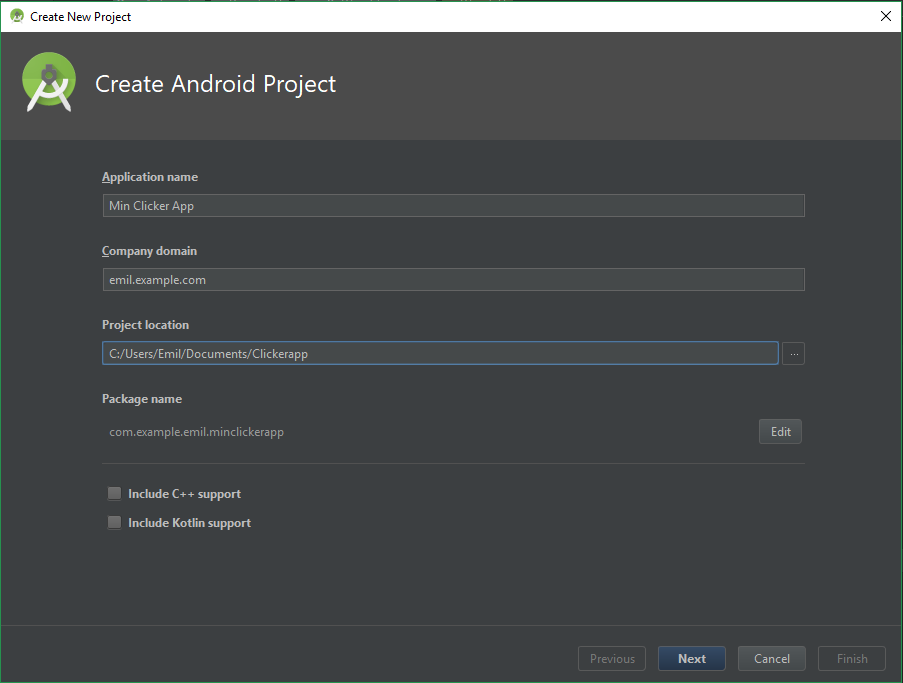
\includegraphics[width=\textwidth]{CreateProject}
	\caption{Eksempel 1.1}
	\label{fig:createproject}
\end{figure}
Det er godt at lave en mappe til sit projekt så man let kan finde det igen. 

Bagefter skal man vælge hvorfor en version af Android den laveste version skal kunne installeres på. Man kan også lave til andre platforme men det vil jeg ikke komme længere ind på. 
\begin{figure}[H]
	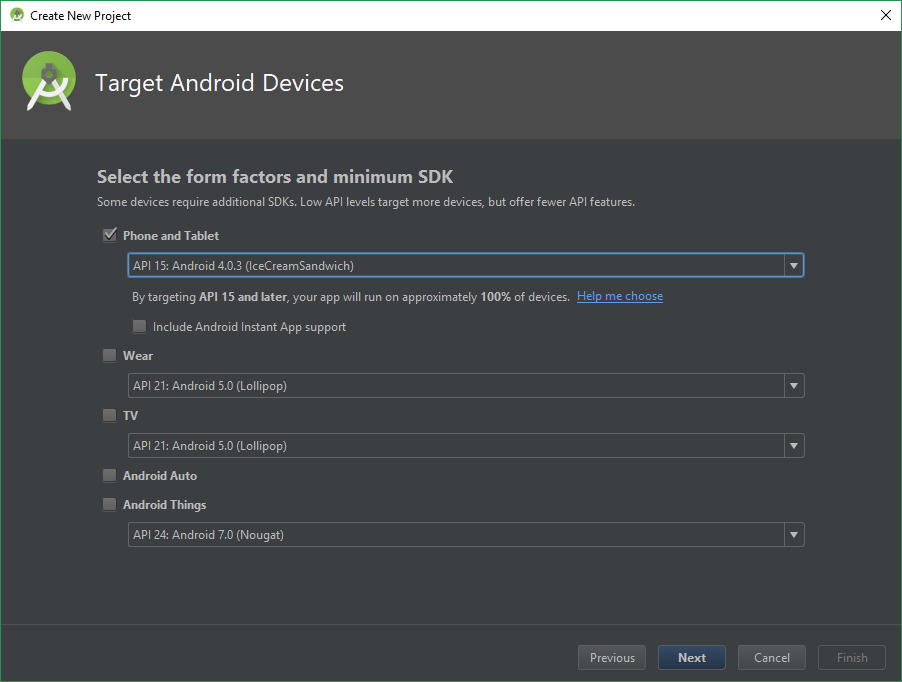
\includegraphics[width=\textwidth]{API}
	\caption{Eksempel 1.2}
	\label{fig:API}
\end{figure}

Derefter skal vælger man Activity
man kan vælge en tom en og starte fra bunden. eller vælge en pre-defineret som jeg har gjort i eksemplet

\begin{figure}[H]
	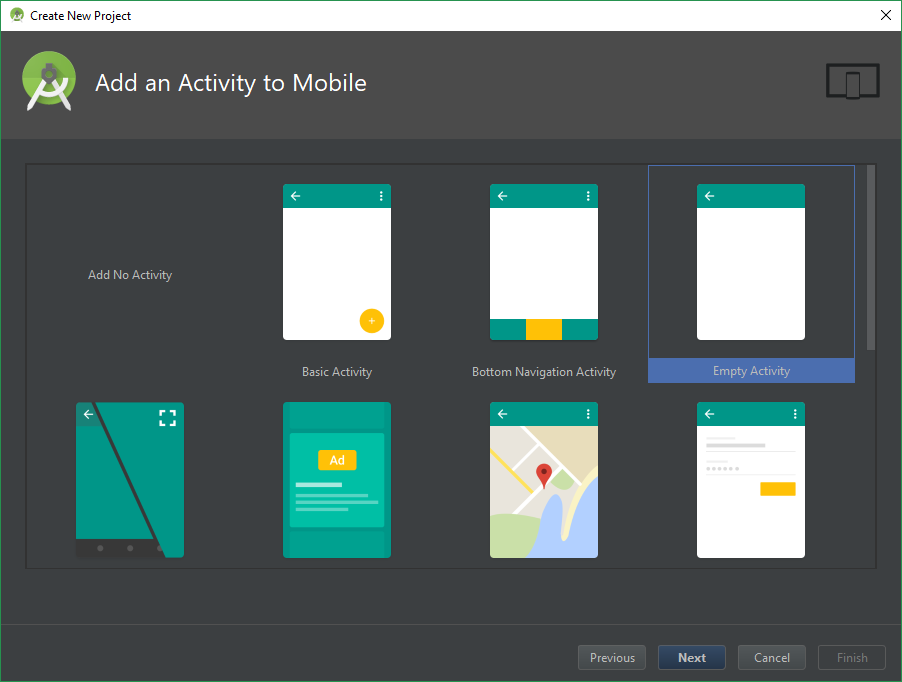
\includegraphics[width=\textwidth]{Activity}
	\caption{Eksempel 1.2}
	\label{fig:Activiy}
\end{figure}

Så skal du navngive din activity, lettest bare lade stå main activitet 

\begin{figure}[H]
	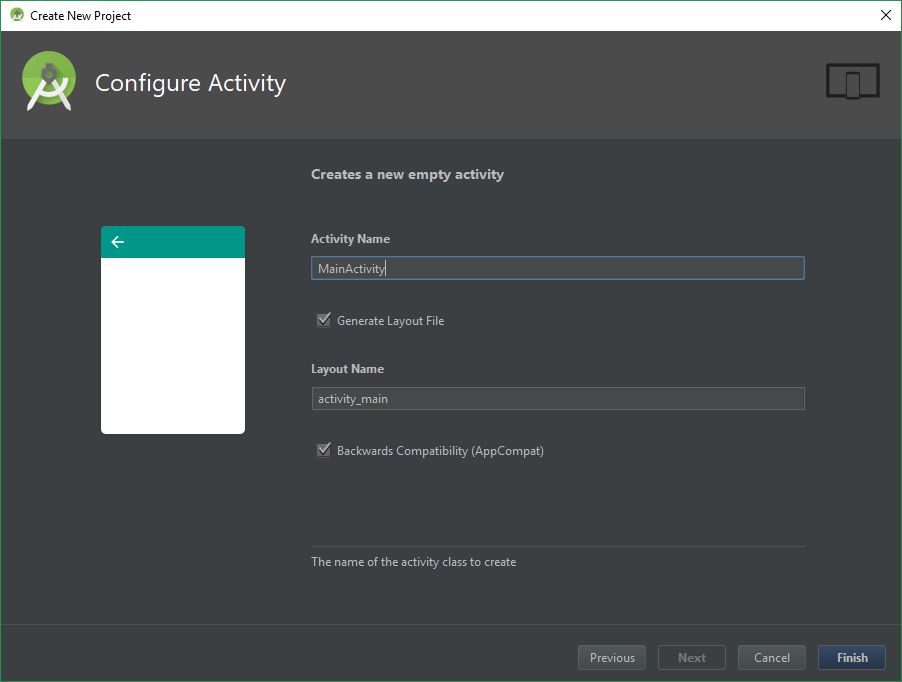
\includegraphics[width=\textwidth]{ConfigActivity}
	\caption{Eksempel 1.2}
	\label{fig:Config Activiy}
\end{figure}

Nu vil Android Studio så sætte basis tingene op. 

\section*{Klikker Spillet}

Nu da vi har fået lavet skelettet til appen skal vi have knapper og text felter

\begin{figure}[H]
	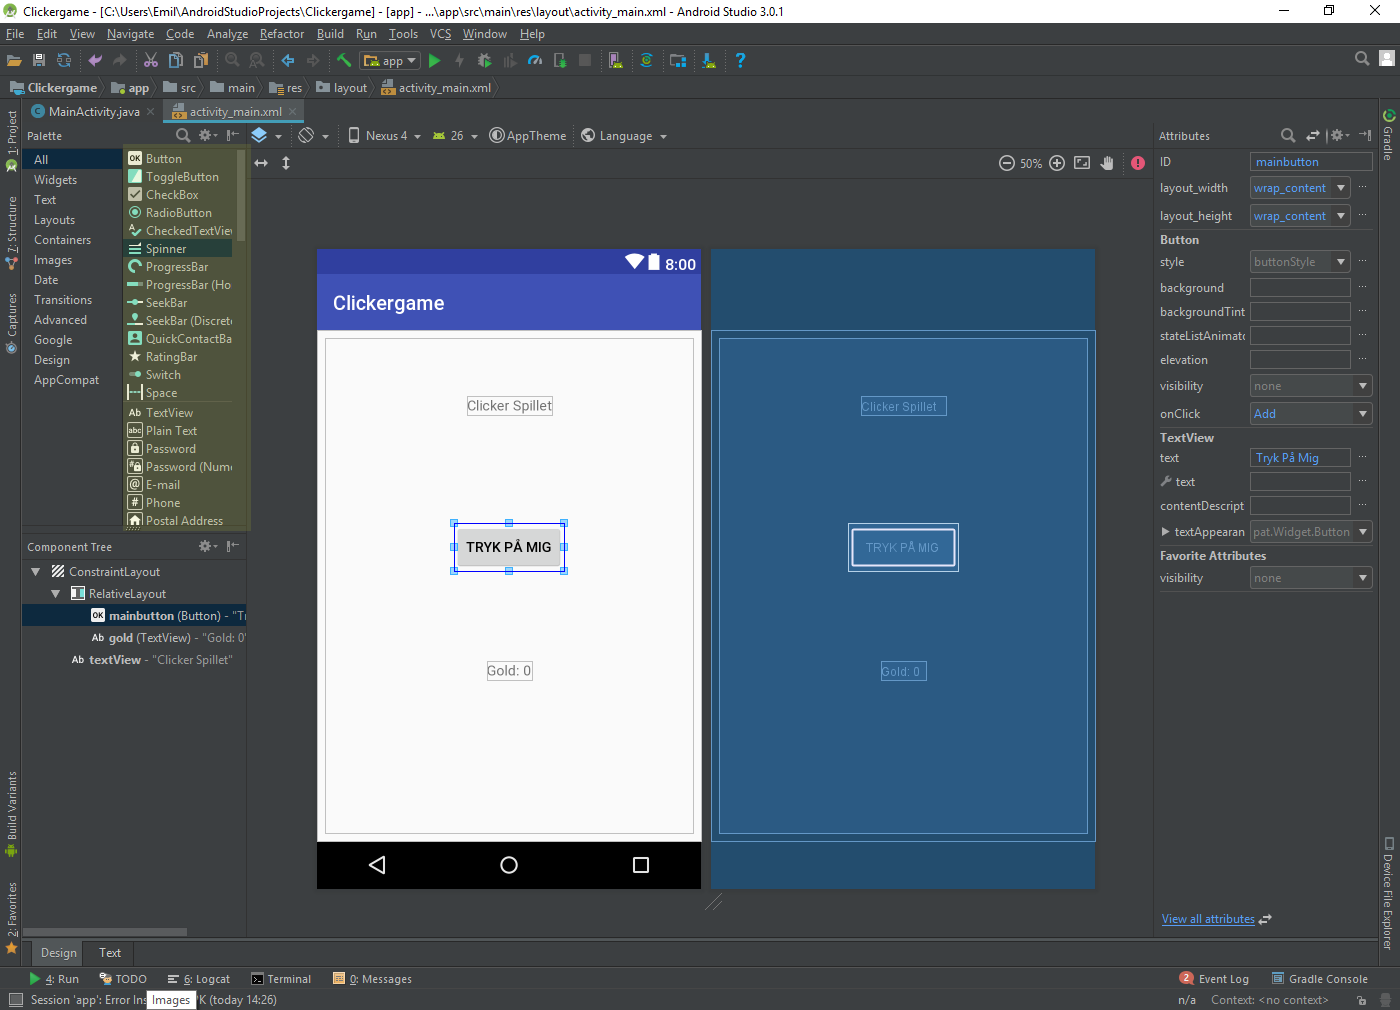
\includegraphics[width=\textwidth]{App}
	\caption{Eksempel 1.1}
	\label{fig:App}
\end{figure}

De findes i paletten som er markeret med gul. 

Tryp på Mig firkanten er en Button og Gold: 0 er et Textview. 
Knapperne og tekst felterne kan ses i component tree i venstre hjørne og der kan du også se hvis du har andre komponenter.

Hvis du har en knap eller et tekstfelt markeret kan du set dets attributes i højre side.

Det er vigtigt at hver knap eller tekst felt har et ID, så det kan findes i koden. Ellers kan du bare rode rundt med de andre. 

Der skulle også være lavet en Mainactivity java fil.

Det her er hvad jeg har skrevet i min activity. 
\begin{figure}[H]
	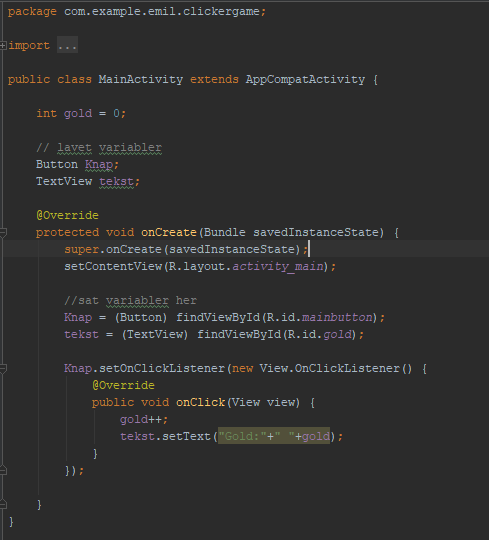
\includegraphics[width=\textwidth]{Java}
	\caption{Eksempel 1.1}
	\label{fig:Java}
\end{figure}

Jeg har sat en variabel gold som har styr på guld beholdningen. 

Derefter har jeg lavet de to variabler Knap og tekst. 

på oncreate, som er når appen starter, har jeg sat den til at finde Knappen og tekst feltet som jeg satte ind. 

Derefter har man brug for en onclicklistener, som opfanger når folk trykker på knappen. 

Så det der sker når folk trykker på knappen er at gold øges med 1 og tekst feltet ændres til Gold og derefter hvor meget huld man har. 

Tilsidst kan appen afprøves på en android mobil eller på en emulator. på mobilen er man nød til at slå filoverførsel til. 







	
	\graphicspath{{sections/android/layouts/figures/}}
	% !TeX spellcheck = da_DK
\chapter{Android udvikling}

Når vi snakker om Android, så snakker vi om et "styresystem". Det kan man 
anskue som et kæmpe stort program, der administrerer alle de apps, der kører på 
mobil-telefonen. I denne bog bruger vi begreberne "styresystem" og "platform" 
i flæng.

De eneste relevante styresystemer til mobiler er, pt., de følgende to:

\begin{itemize}
	\item IOS (IPhone, IPads etc.)
	\item Android (Samsung, HTC, Sony etc.)
\end{itemize}

På SDC kigger vi på den sidste af de to, nemlig Android platformen. Selvom 
app-udvikling til IOS og Android minder meget om hinanden, så er der en række 
væsentlige forskelle i de værktøjer, man bruger. Derfor kigger vi kun på den ene 
af de to styresystemer.

\section{Hvad er Android apps?}

\marginfigure{xkcd_app.png}{Billede lånt af: \url{https://xkcd.com}}

Når man skal beskrive, hvad en ``Android app'' er, så kan det gøres lidt 
simplere ved at forstå hvad en ``app'' er. App er en forkortelse for 
applikation, hvilket i denne kontekst er synonymt med ``et program''. Når vi 
snakker om en app, snakker vi derfor om et computer program, som er kodet med 
en række instruktioner. Derfor er de programmer, du har på din mobil, som 
WordFeud, SnapChat og Facebook, alle eksempler på apps. Computerspil som 
Farming Simulator 2017 og Battlefield 4 er også eksempler på apps, så 
det er faktisk et meget vidt begreb. 

I Android verdenen, er stort set alt apps. Lige fra låseskærmen og 
``indstillinger''-menuen til Super Mario Go, og Farmville. Derfor er der meget 
få grænser for, hvad man kan opnå ved app-udvikling til Android.

\subsection{Anatomien af en Android app}
Android apps består af mange forskellige dele. De primære dele kan dog deles op i følgende tre kategorier:

\subsubsection{Ressourcer}
Ressourcer er indstillinger, billeder, layouts (se \autoref{sec:android:layouts}) og alt muligt andet data, der bruges i en app. De findes i mappen \texttt{res/} og har forskellige undermapper, afhængig af hvilken type ressource det er.

\subsubsection{Activities}
Activities er aktiviteter, man kan foretage sig i app'en. Der kan f.eks. være en "tag billede" activity, en "gem billedet" activity og en "se dit galleri af billeder" activity. Disse activities vil blive udforsket yderligere i \autoref{cha:activities-intents}.

\subsubsection{Manifest}
Et app-manifest er en beskrivelse af app'en som Android styresystemet gør brug af, når den kører app'en på mobilen. I manifestet beskriver man, hvilke rettigheder app'en har brug for, samt hvilke teknologier den gør brug af.

Derudover kan manifestet indeholde information om, hvordan andre apps kan kommunikere med denne app, og andre indstillinger, der binder app'en sammen med resten af platformen.

\section{Layouts}
\label{sec:android:layouts}

Layouts er en ressource som app'en gør brug af, når den skal vise den 
\gls{interface}\footnote{En \gls{interface} er, i denne kontekst, det grafiske 
design, som brugeren interagerer med. Det kan f.eks. være en menu med knapper 
eller et billede.}, som brugeren skal se på inde i app'en. Det er en beskrivelse 
af strukturen i app'ens \gls{interface}.

For bedre at forstå layouts, skal vi først forstå den måde, vi skriver et layout på. Ligesom med programmeringssprog, hvor vi har forskellige sprog til at beskrive kode på (som f.eks. Java), findes der forskellige måder at beskrive strukturer og layouts. Vi kalder disse sprog for \textit{strukturelle sprog}, en af de mere udbredte af sådanne sprog, er det man kalder for \textit{XML}\footnote{e\textbf{X}tensible \textbf{M}arkup \textbf{L}anguage}.

\subsection{XML}
I sin kerne er XML et meget simpelt sprog. Det er bygget op af ``tags'', hvoraf 
der findes to slags tags: et ``opening-tag'' og et ``closing-tag''. 
Opening-tags er skrevet ved, at have et ``mindre-end'' tegn ($<$), efterfulgt af 
noget tekst og så afsluttet med et ``større-end'' tegn ($>$). For eksempel er 
følgende et opening-tag: \XmlInline|<Button>|.

Closing-tags er meget lig opening-tags, der er blot en skråstreg efter 
``mindre-end'' tegnet, for at indikere at dette tag lukker et opening-tag, der 
er skrevet tidligere i dokumentet. Et eksempel på et closing-tag, der lukker 
det opening-tag, der var i det tidligere eksempel, kan ses her: 
\XmlInline|</Button>|.

Det er vigtigt, at man altid lukker sine tags. Man må aldrig have et opening-tag uden, at det bliver lukket, og man må aldrig have et closing-tag, der ikke har noget opening-tag at lukke.

Man kan tilknytte ``attributter'' til sine opening-tags. Det gør man ved at 
skrive navnet på attributten, efterfulgt af et lig-med tegn, efterfulgt af 
attributtens værdi. Denne værdi er typisk skrevet inden i to gåse-øjne ("). Et 
eksempel på et opening-tag med en attribut er følgende: 
\XmlInline|<Button Text="Hej med dig!">|.

Et eksempel på et XML dokument, kan ses i \autoref{lst:first-valid-xml-document}. Det beskriver et vindue med en ``label'' dvs. et kort stykke tekst, med to knapper. Vi har skrevet de tags, der hører til vores label og knapperne imellem vinduets opening- og closing-tags. Dette betyder, at de kommer til at høre til vinduet, altså at vinduet har en label og to knapper. Denne relation bliver ofte beskrevet som, at 
vinduet er forældreren til de tre børn (label og de to knapper).

\begin{example}
	\begin{XmlCode}{Et lille XML dokument}{lst:first-valid-xml-document}
		<Window>
			<Label Text="Vil du lukke vinduet?"></Label>
			<Button Text="Ja"></Button>
			<Button Text="Nej"></Button>
		</Window>
	\end{XmlCode}
\end{example}


For at simplificere XML dokumentet, kan vi udnytte os af et så-kaldt 
self-closing tag. Altså et opening-tag, der lukkes med det samme, uden man 
behøver at bruge et closing-tag. Dette skrives ved at putte en skrå-streg ind 
før ``større-end'' tegnet. Se \autoref{lst:self-closing-tags-document}

\begin{example}
	\begin{XmlCode}{Et lille XML dokument med self-closing tags.}{lst:self-closing-tags-document}
		<Window>
			<Label Text="Vil du lukke vinduet?"/>
			<Button Text="Ja"/>
			<Button Text="Nej"/>
		</Window>
	\end{XmlCode}
\end{example}

\begin{remark}
	Bemærk at vi ikke kunne bruge et self-closing tag til vores \XmlInline|<Window>| tag, fordi det ikke skulle lukkes med det samme, da det skulle indeholde dets tre børn.
\end{remark}

Vi har nu taget en kort intro til XML, det er faktisk et meget mere komplekst sprog, end det, vi har gennemgået her, men det burde ikke blive nødvendigt, at forstå det hele for det vi skal arbejde med her.

Hvis man gerne vil lære mere om XML, kan man besøge W3Schools: \url{https://www.w3schools.com/xml/}.

\subsection{Views}
Et view er så et af de elementer som brugerfladen er bygget af. En knap er et view. Et stykke tekst er et view. Et billede er et view. I kan finde alle de forskellige elementer i menuen som er markeret med en rød grænse i \autoref{fig:android:layouts:viewmenu}

\begin{figure}[h]
	\begin{center}
		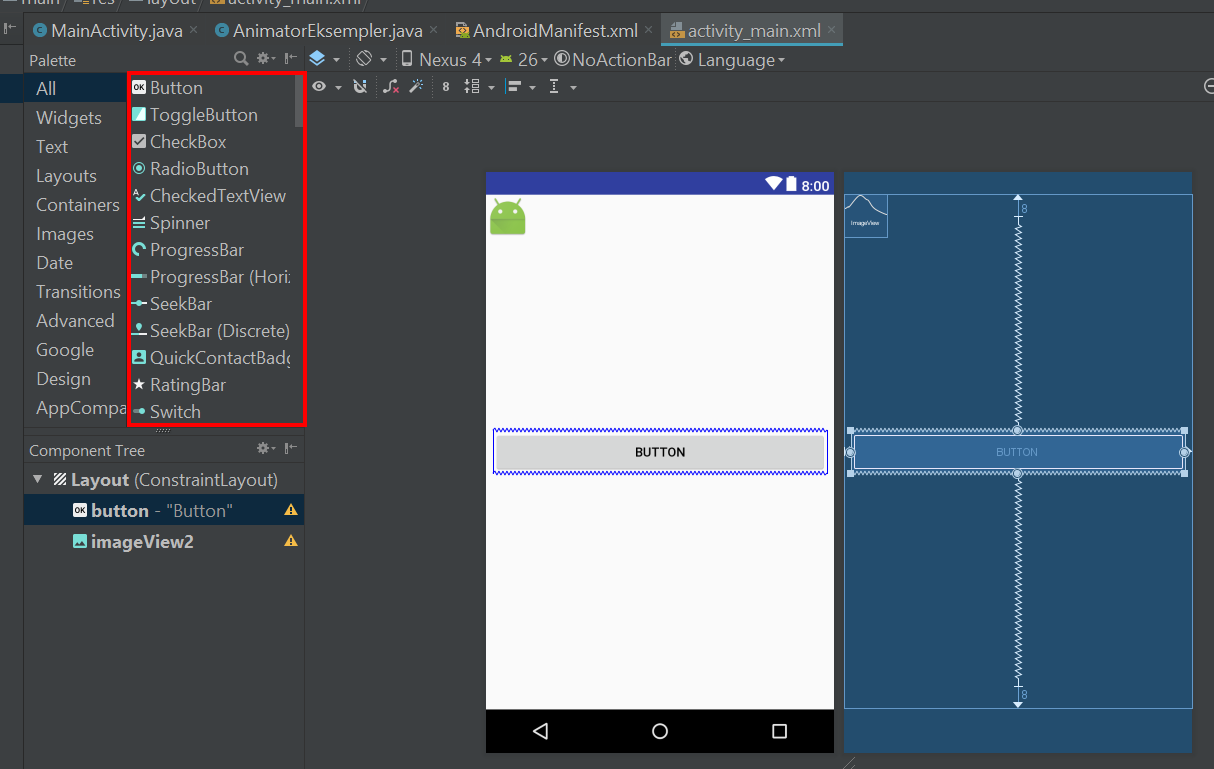
\includegraphics[width=5cm]{view_menu.png}
		\caption{menuen med views}
		\label{fig:android:layouts:viewmenu}
	\end{center}
\end{figure}

Man kan specificere egenskaberne (properties) på elementerne ved at flytte på elementerne i Design tabben, eller specificere egenskaberne i XML filen. For størrelsen af viewet kan man anvende:
\begin{itemize}
	\item wrap\_content , som fortæller dit view at det skal reguleres efter den størrelse som er fastsat af indholdet (evt. teksten på en knap).
	\item match\_parent , som fylder det viewet er indeni ud.\\
	\item density-independent pixels (dp) , er en relativ størrelse som kan sættes for at nærmere præcisere lokationen på dit element, eksempelvis højden, bredden, relationen til andre elementer (hvis du bruger relative layout).
\end{itemize}

Vi kommer ind på hvordan du bruger programmering til at ændre på hvordan dine views ser ud (såsom teksten) i næste kapitel.

\subsection{Hvad er layouts?}
Layouts er, som nævnt, en måde at beskrive app'ens udseende på igennem det strukturelle sprog XML. Layouts er også de elementer man bruger til at organisere views. Så hvis man vil have nogle views til at sidde på en speciel måde ligger man dem ind i et layout.

Vi lægger layouts i ressource mappen \texttt{res/layout/}, og et layout er 
faktisk bare et XML-tag, der kan indeholde andre tags som repræsenterer views.

I Android Studio er der mulighed for, at arbejde med disse layouts igennem en 
visuel editor, så man slipper for at rode med XML-kode. Det er dog stadig en 
god idé, at forstå hvordan de fungerer i koden, både for forståelsens skyld og 
for at kunne rette fejl, hvis det visuelle redigeringsværktøj driller.

\subsubsection{Frame layouts}

Det første eksempel på et layout, er det såkaldte \textit{frame layout}, det er et meget simpelt og effektivt layout, der er designet til at pladsere et enkelt element et specifikt sted på skærmen.

Det er svært at håndtere dette layout, hvis det har mere end et barn. Derfor bør 
det typisk kun indeholde et enkelt barn. Deraf kommer navnet ``frame'', det 
bruges som en ``ramme'' til et andet element.

I \autoref{fig:android:layouts:frame-layout} er der et eksempel på, hvordan man 
kan have to ``børn'' indeni et frame layout, for at placere det ene oven på det 
andet.

\begin{figure}[h]
	\begin{center}
		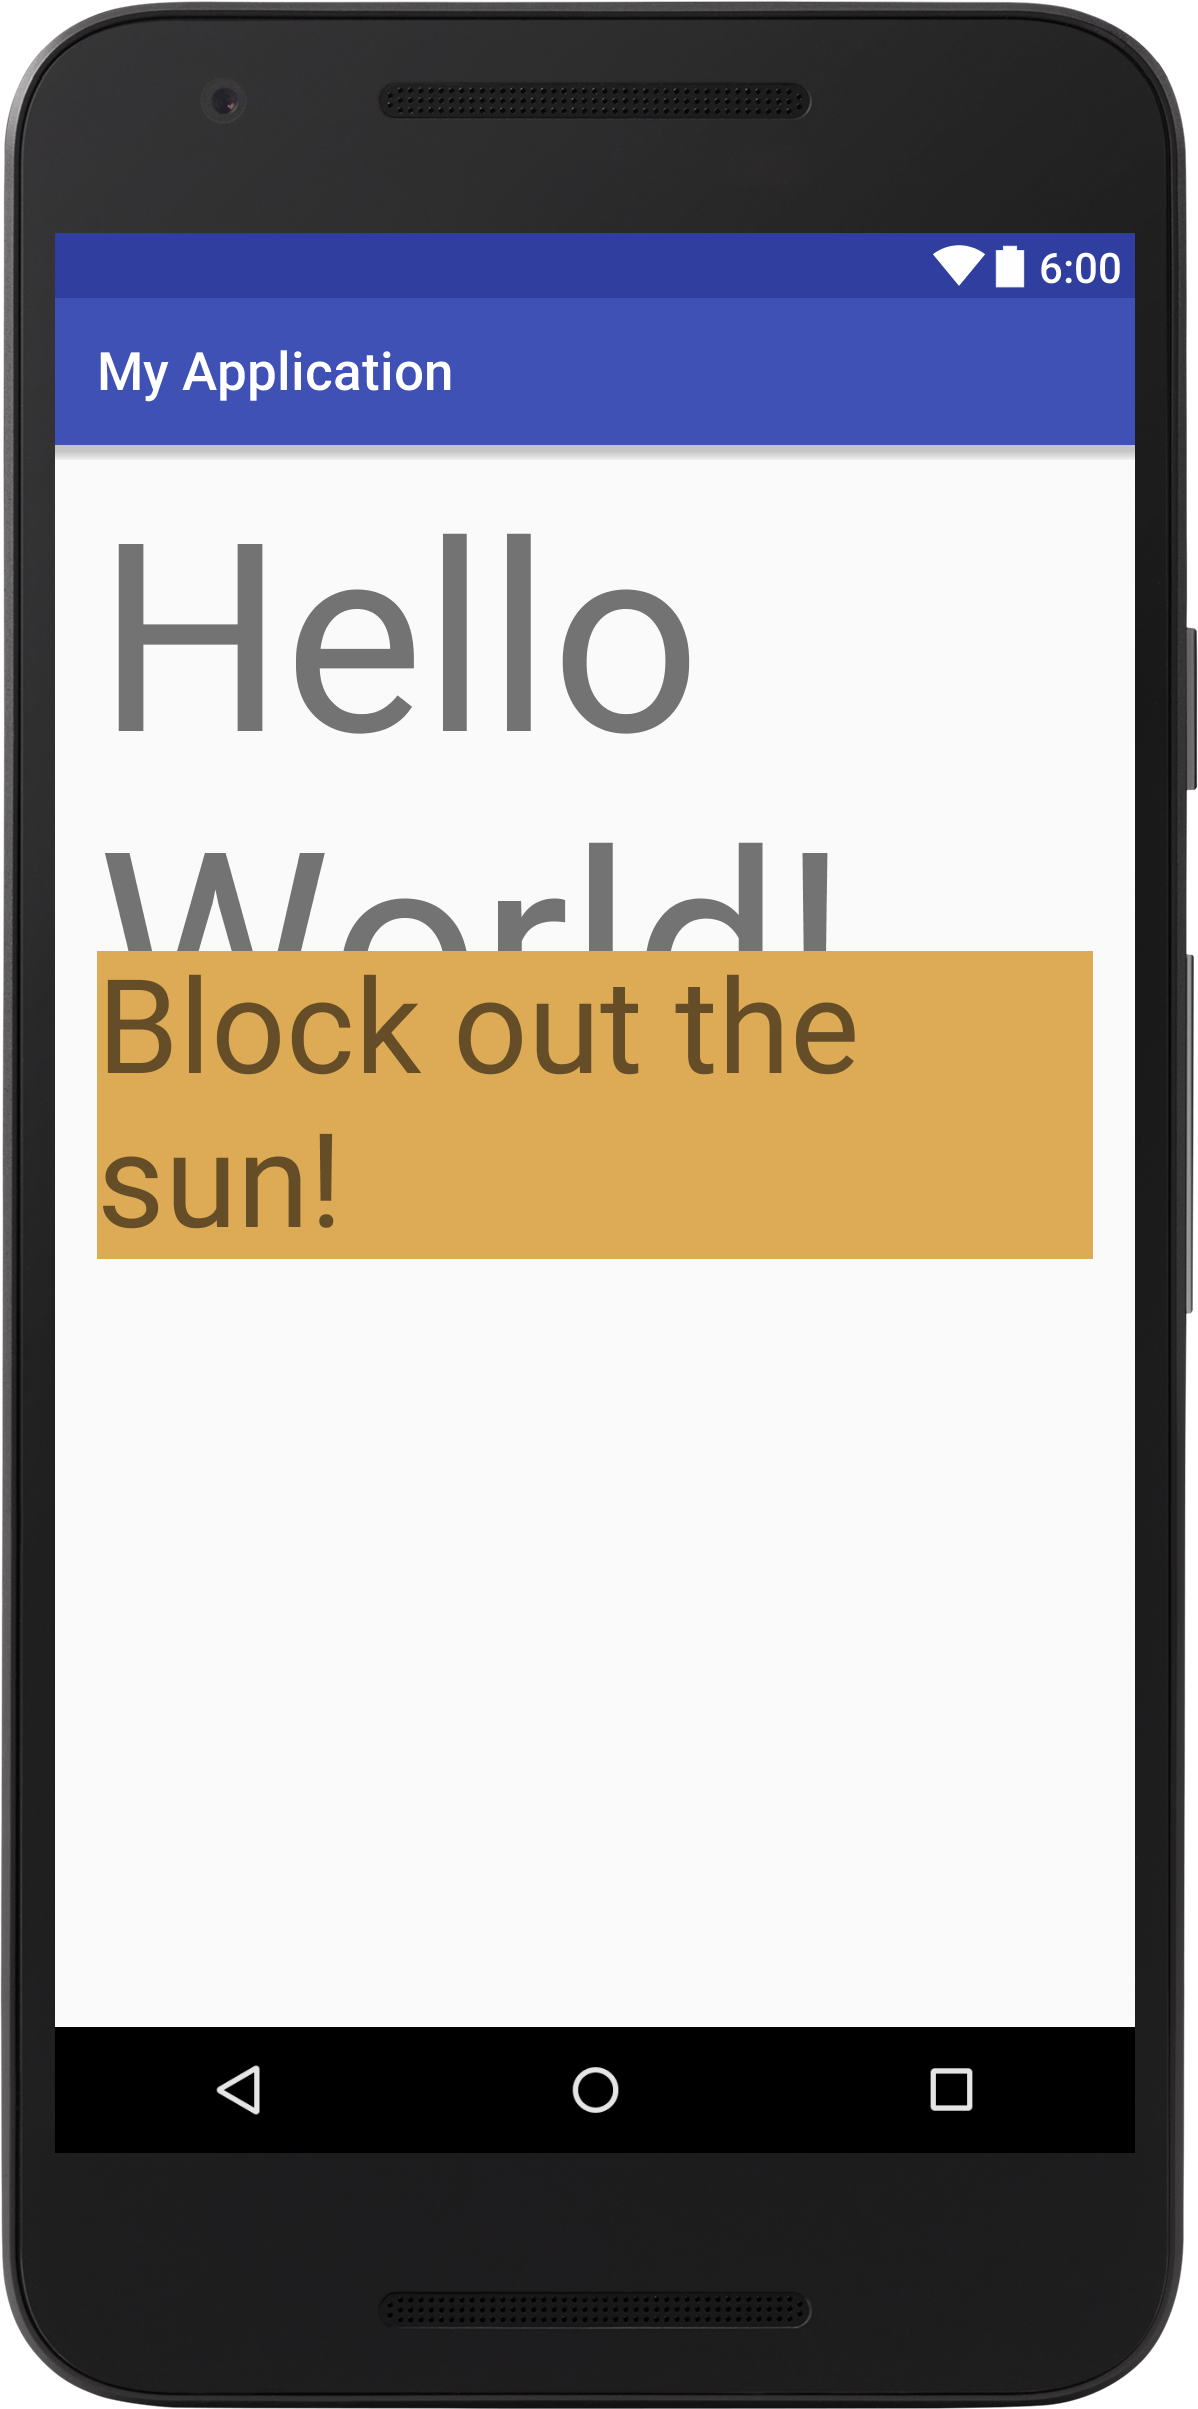
\includegraphics[width=5cm]{frame_layout.png}
		\caption{Et frame layout i en app.}
		\label{fig:android:layouts:frame-layout}
	\end{center}
\end{figure}

\begin{XmlCode}{Det layout, der giver udseendet i \autoref{fig:android:layouts:frame-layout}}{lst:frame-layout}
	<?xml version="1.0" encoding="utf-8"?>
	<FrameLayout 
		xmlns:android=
			"http://schemas.android.com/apk/res/android"
		xmlns:tools="http://schemas.android.com/tools"
		android:layout_width="match_parent"
		android:layout_height="match_parent"
		android:paddingBottom=
			"@dimen/activity_vertical_margin"
		android:paddingLeft=
			"@dimen/activity_horizontal_margin"
		android:paddingRight=
			"@dimen/activity_horizontal_margin"
		android:paddingTop=
			"@dimen/activity_vertical_margin"
		tools:context=
			"com.example.lukas.myapplication.MainActivity">
	
		<TextView
			android:layout_width="wrap_content"
			android:layout_height="wrap_content"
			android:text="Hello World!"
			android:textSize="100sp"/>
		<TextView
			android:layout_width="fill_parent"
			android:layout_height="wrap_content"
			android:layout_gravity="center_vertical"
			android:layout_marginBottom="50dp"
			android:background="#ddaa55"
			android:text="Block out the sun!"
			android:textSize="50sp"/>
	</FrameLayout>
\end{XmlCode}

\clearpage
\FloatBarrier

\subsubsection{Linear layouts}
Linear layouts er det simpleste layout, man kan bruge. Det tager alle sine 
børn, og arrangerer dem således, at de ligger enten under hinanden (vertikalt) 
eller ved siden af hinanden (horisontalt).

Der er ikke meget, der kan ændre på, hvordan dette layout virker, men det er 
rigtig simpelt til at vise f.eks. lister eller at pladsere elementer ved siden 
af hinanden.

I \autoref{fig:android:layouts:linear-layout} er der et eksempel på et lineært 
layout med tre børn, det første er bare sat ind og ligger øverst. Det næste er 
sat til at være lige så bredt som skærmen, og bliver automatisk sat nedenunder 
det første. Til sidst fylder det nederste og sidste element resten af skærmen.

\begin{figure}[h]
	\begin{center}
		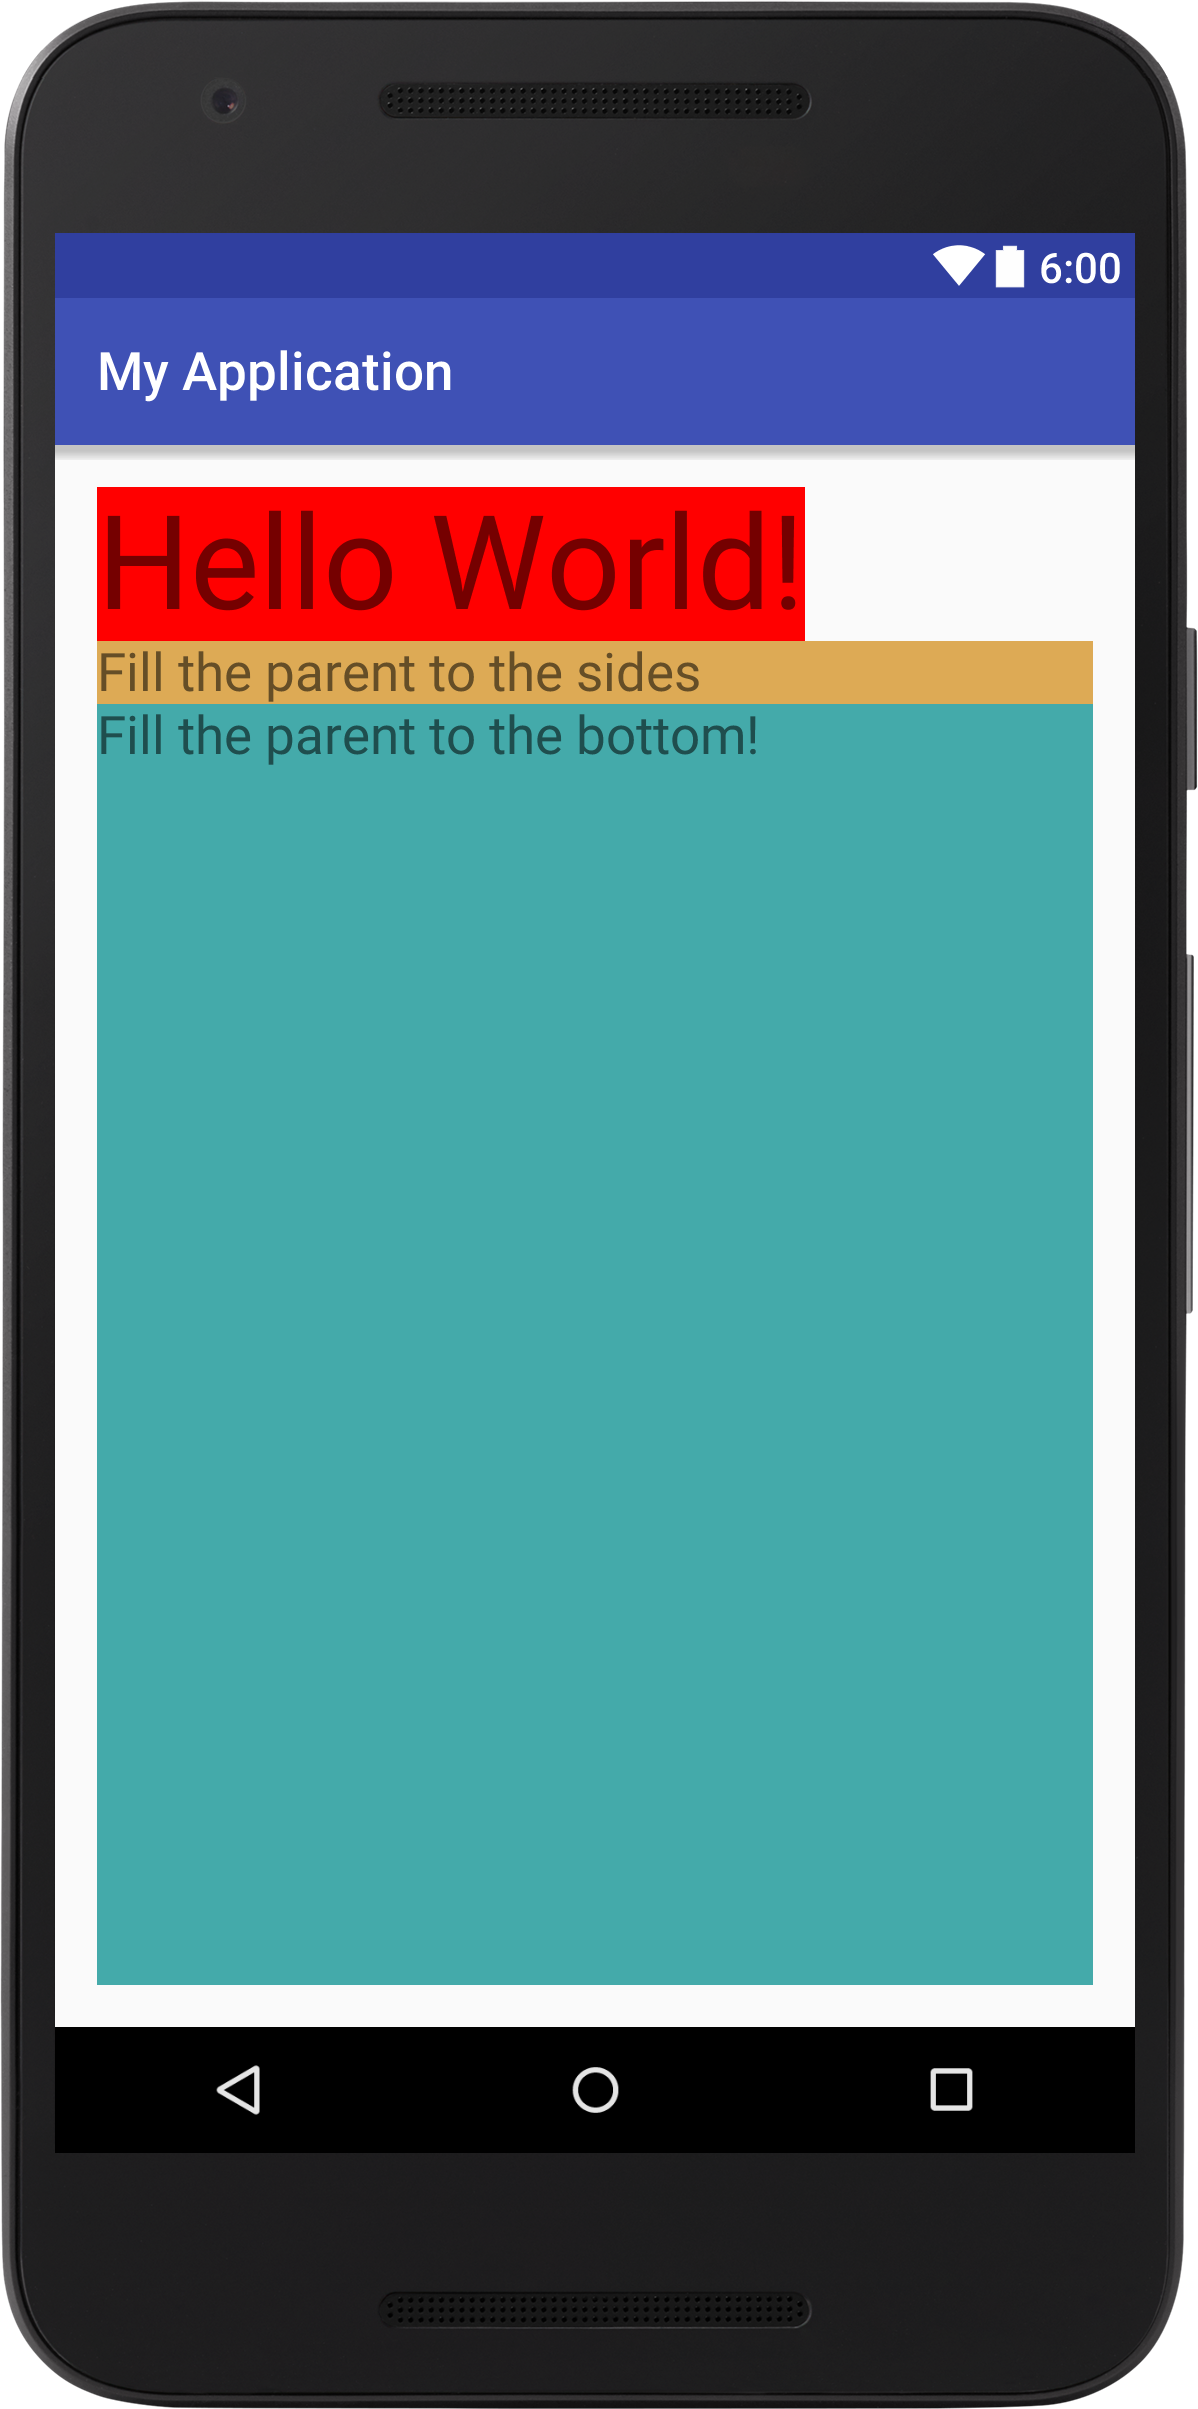
\includegraphics[width=5cm]{linear_layout.png}
		\caption{Et lineært layout i en app.}
		\label{fig:android:layouts:linear-layout}
	\end{center}
\end{figure}

\begin{XmlCode}{Det layout, der giver udseendet i %
\autoref{fig:android:layouts:linear-layout}}{linear-layout}
	<?xml version="1.0" encoding="utf-8"?>
	<LinearLayout 
		xmlns:android=
			"http://schemas.android.com/apk/res/android"
		xmlns:tools="http://schemas.android.com/tools"
		android:layout_width="match_parent"
		android:layout_height="match_parent"
		android:orientation="vertical"
		android:paddingBottom=
			"@dimen/activity_vertical_margin"
		android:paddingLeft=
			"@dimen/activity_horizontal_margin"
		android:paddingRight=
			"@dimen/activity_horizontal_margin"
		android:paddingTop=
			"@dimen/activity_vertical_margin"
		tools:context=
			"com.example.lukas.myapplication.MainActivity">
		
		<TextView
			android:layout_width="wrap_content"
			android:layout_height="wrap_content"
			android:text="Hello World!"
			android:background="#FF0000"
			android:textSize="50sp"/>
		<TextView
			android:layout_width="fill_parent"
			android:layout_height="wrap_content"
			android:background="#ddaa55"
			android:text="Fill the parent to the sides"
			android:textSize="20sp"/>
		<TextView
			android:layout_width="fill_parent"
			android:layout_height="fill_parent"
			android:layout_gravity="center_vertical"
			android:background="#44aaaa"
			android:text="Fill the parent to the bottom!"
			android:textSize="20sp"/>
	</LinearLayout>
\end{XmlCode}

\clearpage

\FloatBarrier
\subsubsection{Table layouts}
Table layouts arrangerer sine børn i rækker og kolonner. De er simple at 
bruge, og er rigtig gode, hvis man skal have noget, der ligner en tabel, men de er 
meget rigide. Alt man laver med tabular-layout, vil se ud som en tabel.
 
I \autoref{fig:android:layouts:table-layout} er der et eksempel på et table 
layout. Der er 3 rækker og 3 kolonner i layoutet. Man laver nye rækker ved at 
putte det, der skal være i rækken inden i et ``TableRow'' tag.
 
\begin{figure}[h]
	\begin{center}
		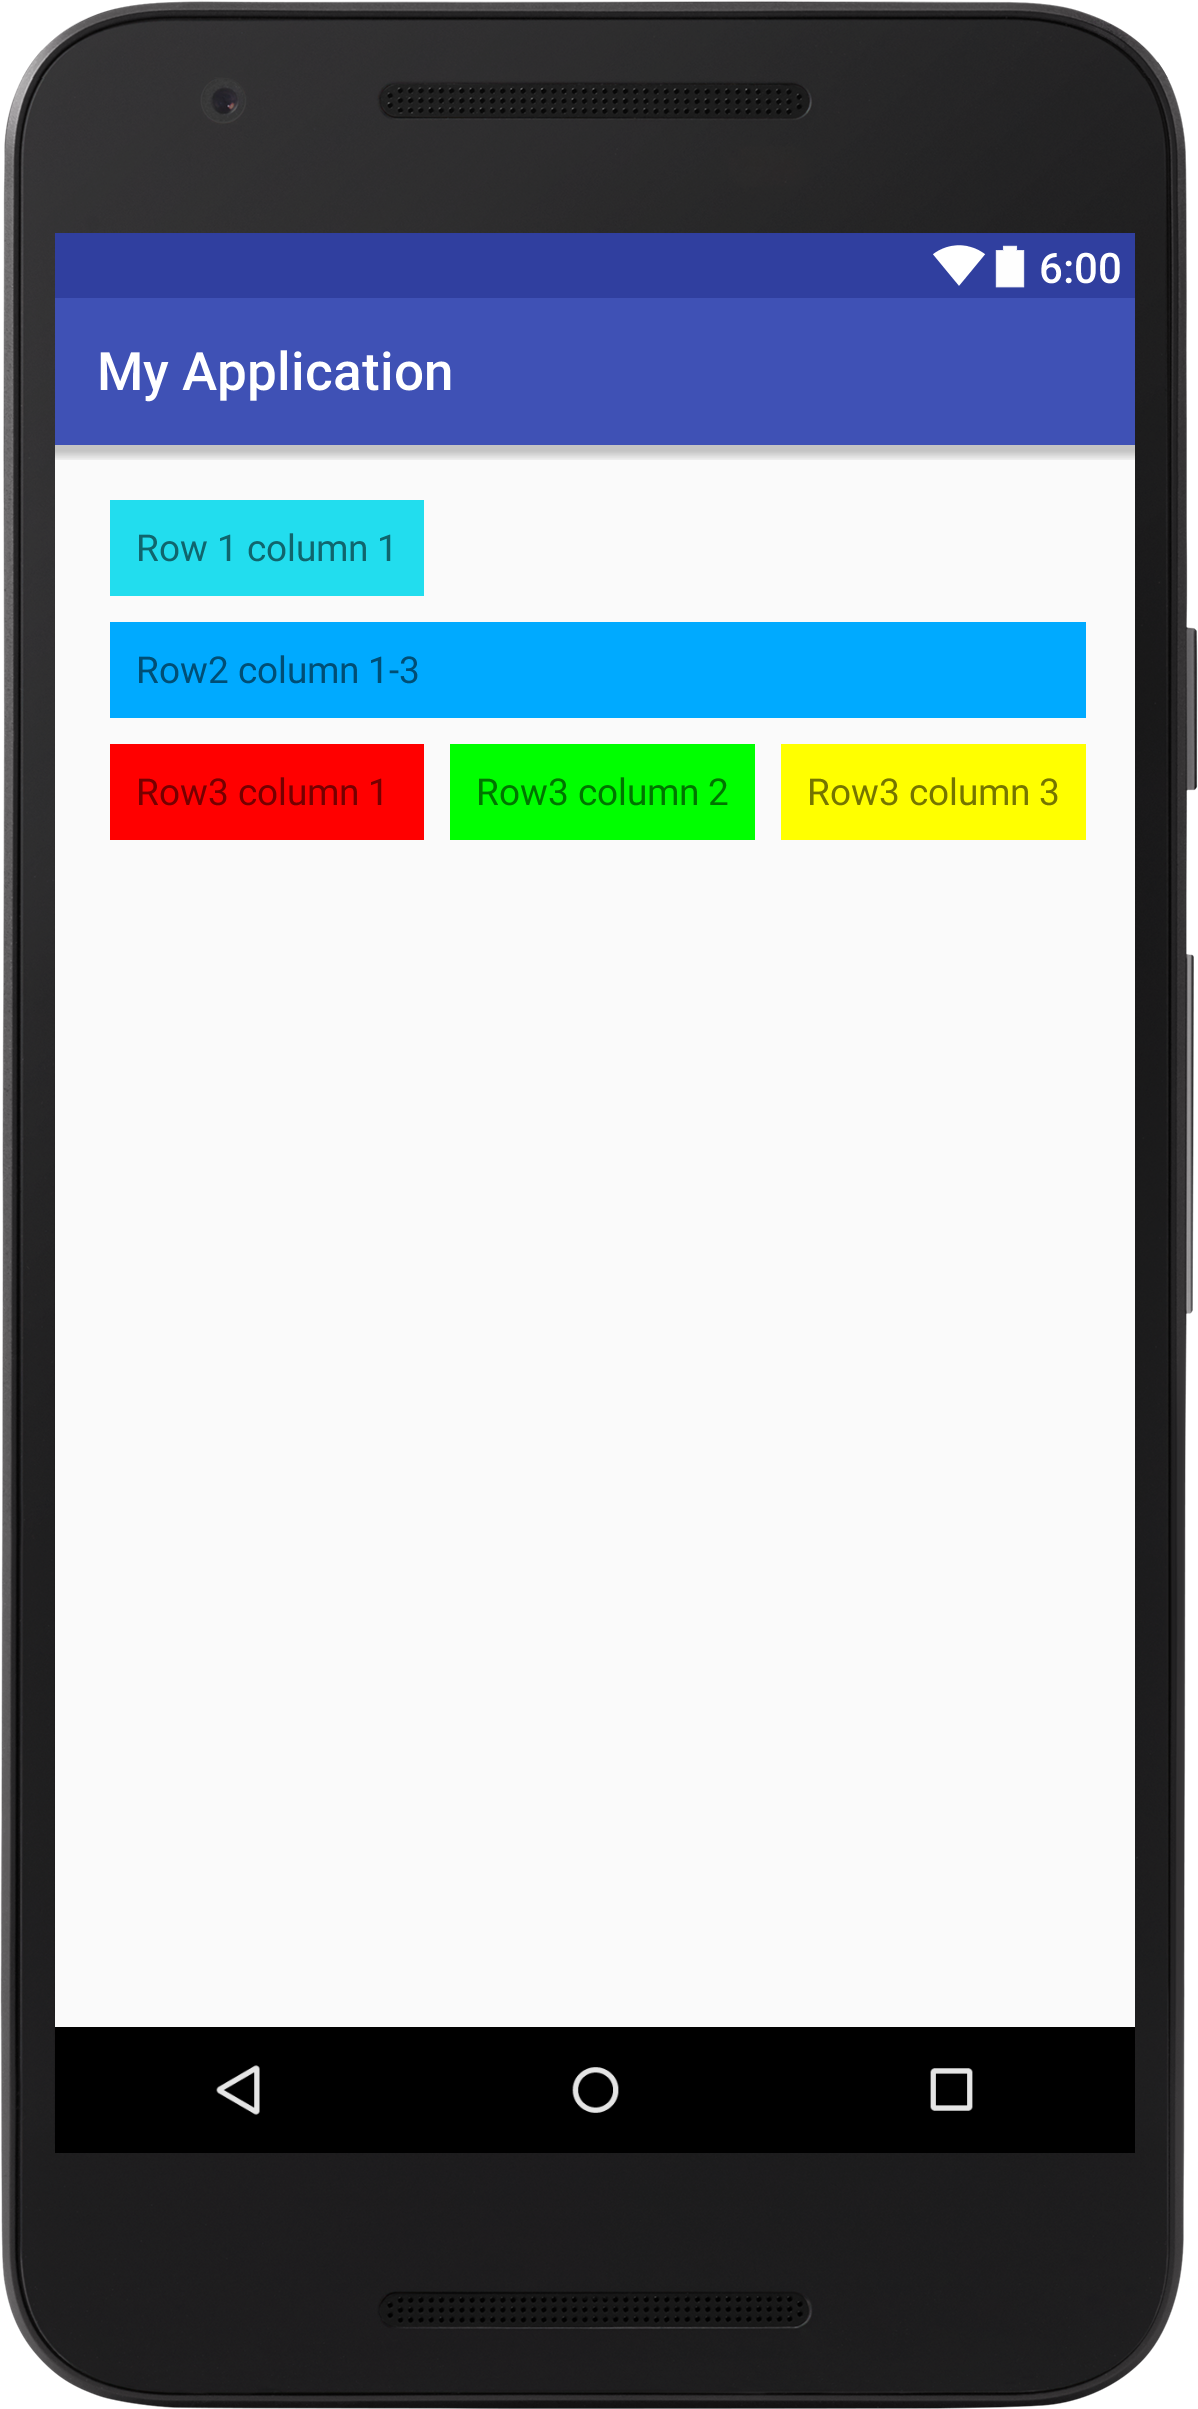
\includegraphics[width=5cm]{table_layout.png}
		\caption{Et table layout i en app}
		\label{fig:android:layouts:table-layout}
	\end{center}
\end{figure}
 
\begin{XmlCode}{Det layout der giver udseendet i %
 		\autoref{fig:android:layouts:table-layout}}{lst:linear-layout}
	<?xml version="1.0" encoding="utf-8"?>
	<TableLayout 
		xmlns:android=
			"http://schemas.android.com/apk/res/android"
		xmlns:tools=
			"http://schemas.android.com/tools"
		android:layout_width="match_parent"
		android:layout_height="match_parent"
		android:paddingBottom=
			"@dimen/activity_vertical_margin"
		android:paddingLeft=
			"@dimen/activity_horizontal_margin"
		android:paddingRight=
			"@dimen/activity_horizontal_margin"
		android:paddingTop=
			"@dimen/activity_vertical_margin"
		tools:context=
			"com.example.lukas.myapplication.MainActivity">
		
		<TableRow>
			<TextView
			android:text="Row 1 column 1"
			android:background="#22ddee"
			android:padding="10dp"
			android:layout_margin="5dp"/>
		</TableRow>
		
		<TableRow>
			<TextView
			android:text="Row2 column 1-3"
			android:background="#00AAFF"
			android:padding="10dp"
			android:layout_span="3"
			android:layout_margin="5dp"/>
		</TableRow>
		
		<TableRow>
			<TextView
			android:text="Row3 column 1"
			android:background="#FF0000"
			android:padding="10dp"
			android:layout_margin="5dp"/>
			<TextView
			android:text="Row3 column 2"
			android:background="#00FF00"
			android:padding="10dp"
			android:layout_margin="5dp"/>
			<TextView
			android:text="Row3 column 3"
			android:background="#FFFF00"
			android:padding="10dp"
			android:layout_margin="5dp"/>
		</TableRow>
	</TableLayout>
\end{XmlCode}

\begin{exercise}
	Lav et tabular-lignende layout ved hjælp af linear layouts.
\end{exercise}

\begin{exercise}
	Lav et linear-lignende layout ved hjælp af tabular layouts (både horisontalt og vertikalt).
\end{exercise}

\clearpage

\FloatBarrier
\subsubsection{Relative layouts}
Relative layouts er et meget fleksibelt og stærkt værktøj. De kan arrangere 
deres børn relativt til hinanden. F.eks. får man mulighed for at sige ``den 
røde kasse skal være til højre for den blå kasse''. Der er næsten ikke det, man 
ikke kan med relative layouts.

\begin{figure}[h]
	\begin{center}
		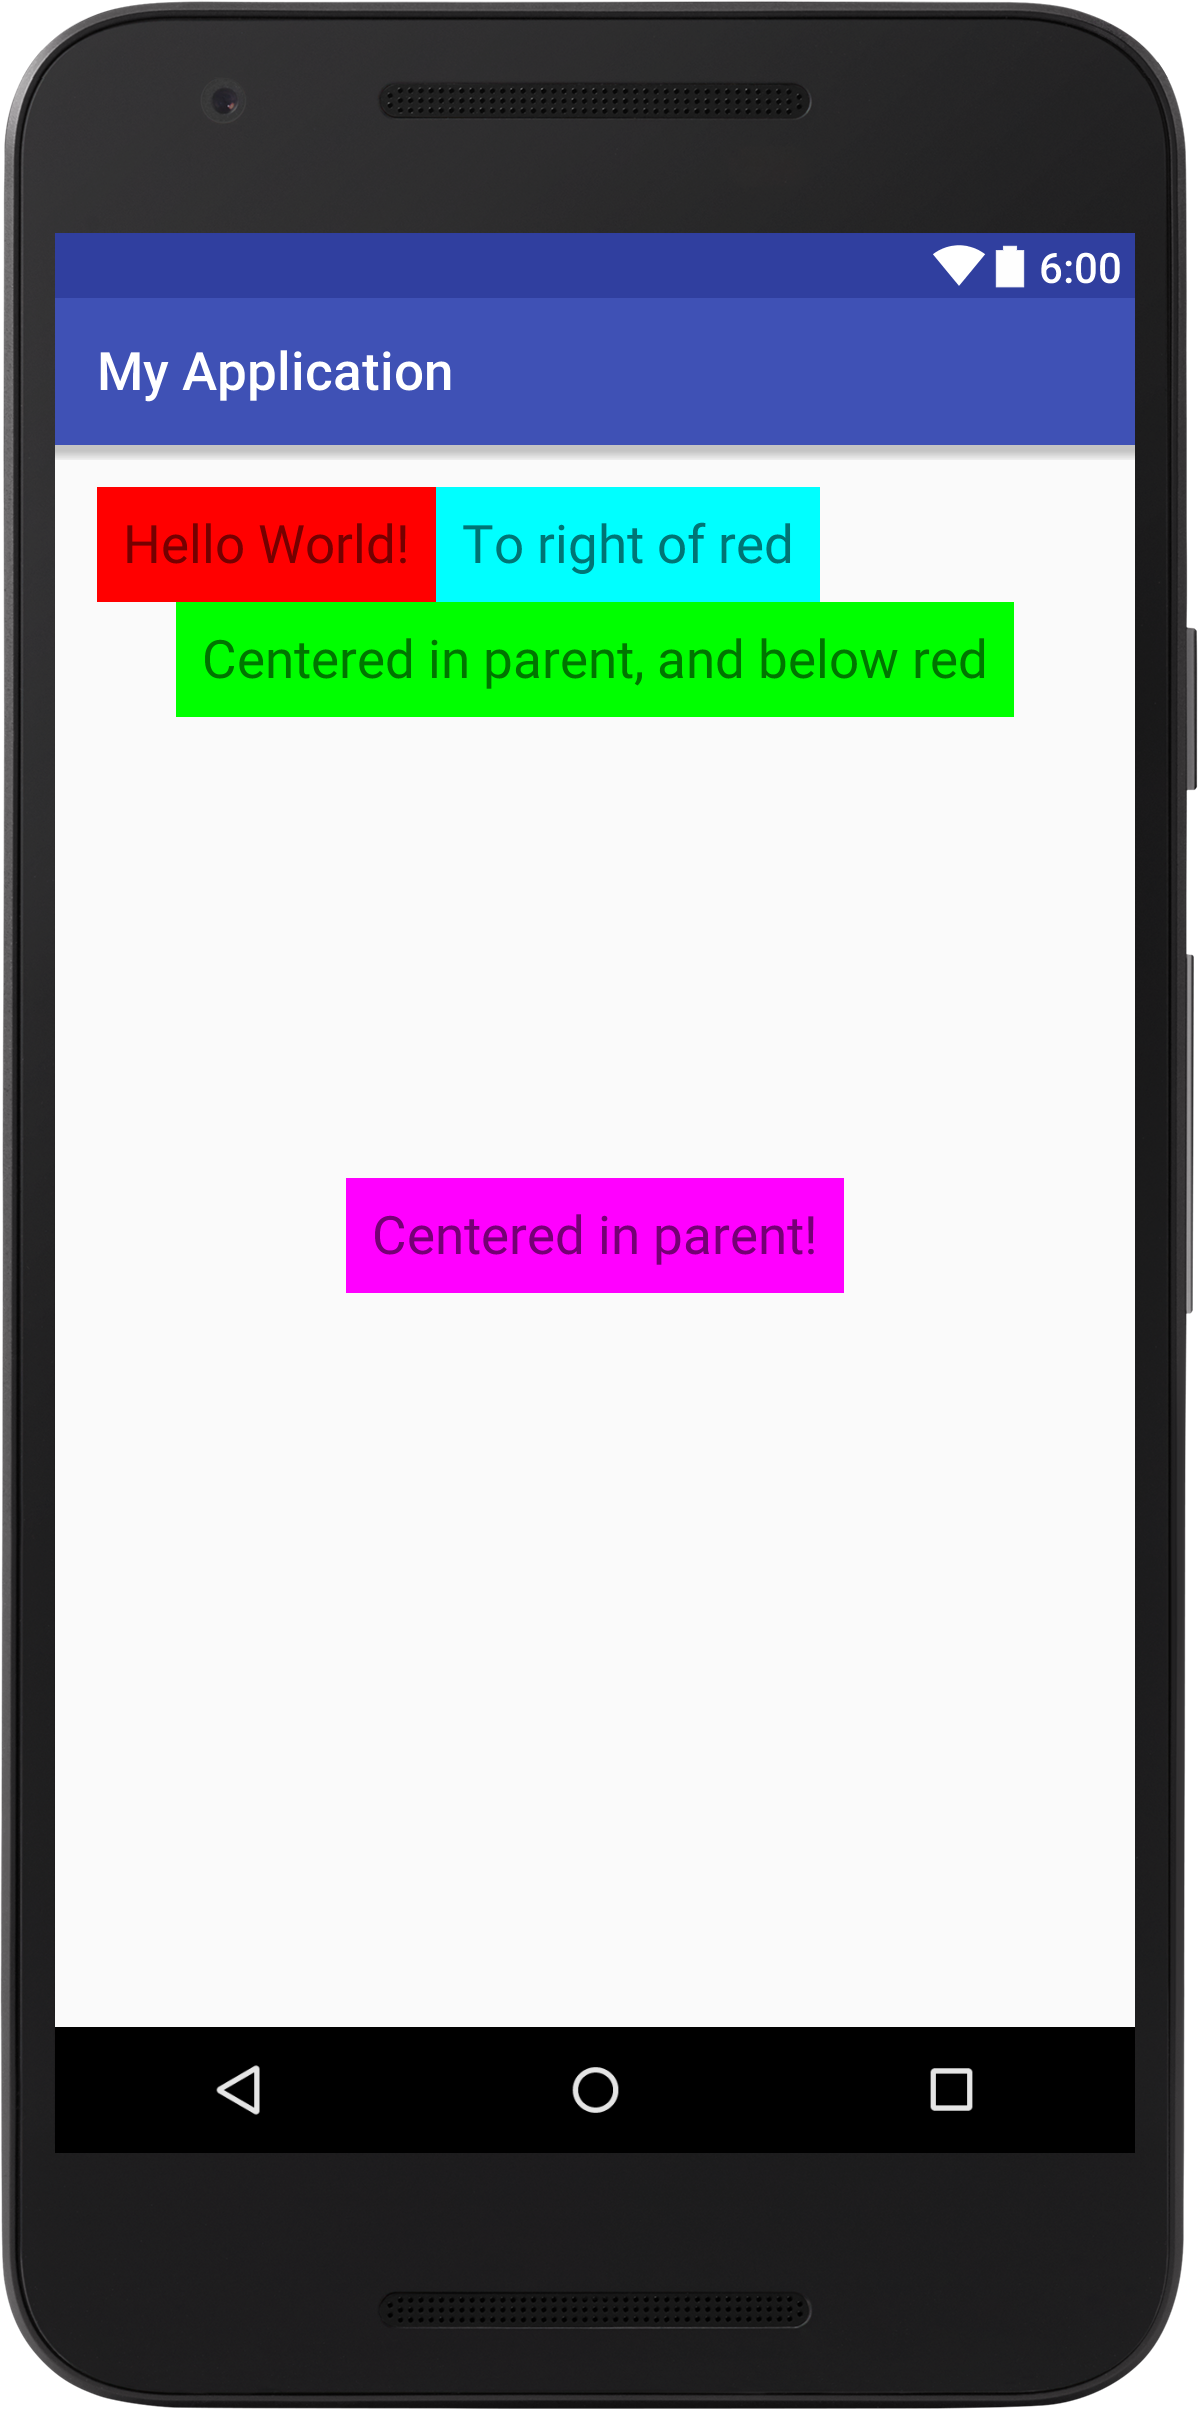
\includegraphics[width=5cm]{relative_layout.png}
		\caption{Et relative layout i en app.}
		\label{fig:android:layouts:relative-layout}
	\end{center}
\end{figure}

\begin{XmlCode}{Det layout der giver udseendet i %
		\autoref{fig:android:layouts:relative-layout}}{lst:relative-layout}
	<?xml version="1.0" encoding="utf-8"?>
	<RelativeLayout 
		xmlns:android=
			"http://schemas.android.com/apk/res/android"
		xmlns:tools=
			"http://schemas.android.com/tools"
		android:layout_width="match_parent"
		android:layout_height="match_parent"
		android:paddingBottom=
			"@dimen/activity_vertical_margin"
		android:paddingLeft=
			"@dimen/activity_horizontal_margin"
		android:paddingRight=
			"@dimen/activity_horizontal_margin"
		android:paddingTop=
			"@dimen/activity_vertical_margin"
		tools:context=
			"com.example.lukas.myapplication.MainActivity">
		
		<TextView
			android:id="@+id/text1"
			android:layout_width="wrap_content"
			android:layout_height="wrap_content"
			android:text="Hello World!"
			android:textSize="20dp"
			android:padding="10dp"
			android:background="#FF0000"
			android:layout_toRightOf="@id/text1"/>
		<TextView
			android:layout_width="wrap_content"
			android:layout_height="wrap_content"
			android:text="Centered in parent, and below red"
			android:textSize="20dp"
			android:padding="10dp"
			android:background="#00FF00"
			android:layout_below="@id/text1"
			android:layout_centerInParent="true"/>
		<TextView
			android:layout_width="wrap_content"
			android:layout_height="wrap_content"
			android:text="Centered in parent!"
			android:textSize="20dp"
			android:padding="10dp"
			android:background="#FF00FF"
			android:layout_centerInParent="true"/>
		<TextView
			android:layout_width="wrap_content"
			android:layout_height="wrap_content"
			android:text="To right of red"
			android:textSize="20dp"
			android:padding="10dp"
			android:background="#00FFFF"
			android:layout_toRightOf="@id/text1"/>
	</RelativeLayout>
\end{XmlCode}

\cleardoublepage

\FloatBarrier
\section{Listeners}
I Android app-udvikling findes der noget, der hedder en ``listener'', som navnet 
antyder, så er der tale om noget, der lytter. I app'ens \gls{interface}, er der 
tale om elementer, der lytter efter brugerens input. F.eks. hvis man gerne vil 
skrive noget kode, der reagerer på, at brugeren trykker på en knap, er der tale 
om en ``On-Click-Listener''.

Disse listeners er altså måden, hvorpå vi kan knytte vores \gls{interface} 
sammen med den kode, vi gerne vil køre. Indtil videre har vi kun snakket om 
layouts, hvordan de virker og ser ud. I praksis er et layout næsten altid 
knyttet sammen med en Activity, som vi snakker mere om i 
\autoref{cha:activities-intents}. Lad os, indtil videre antage at der kun er et 
layout (activity\_main.xml) og én activity (MainActivity.java). Hvis vi ikke 
har ændret i vores Activity, men blot bruger den Activity, som Android Studio 
har lavet til os, vil koden se således ud:

\begin{JavaCode}{En tom MainActivity}{main-activity}
	public class MainActivity extends AppCompatActivity {
		
		@Override
		protected void onCreate(Bundle savedInstanceState) {
			super.onCreate(savedInstanceState);
			setContentView(R.layout.activity_main);
		}
	
	}
\end{JavaCode}

Læg mærke til dette stykke kode: 
\JavaInline|setContentView(R.layout.activity_main)|. I den linje knytter vi 
vores layout (activity\_main.xml) sammen med vores MainActivity, ved at sætte 
MainActivity's indhold til at være activity\_main layoutet.

Vi kan nu ændre vores activity\_main layout, ved at tilføje en knap i midten af 
skærmen, som vist i \autoref{fig:android:layouts:button-layout}.

\begin{figure}[h]
	\begin{center}
		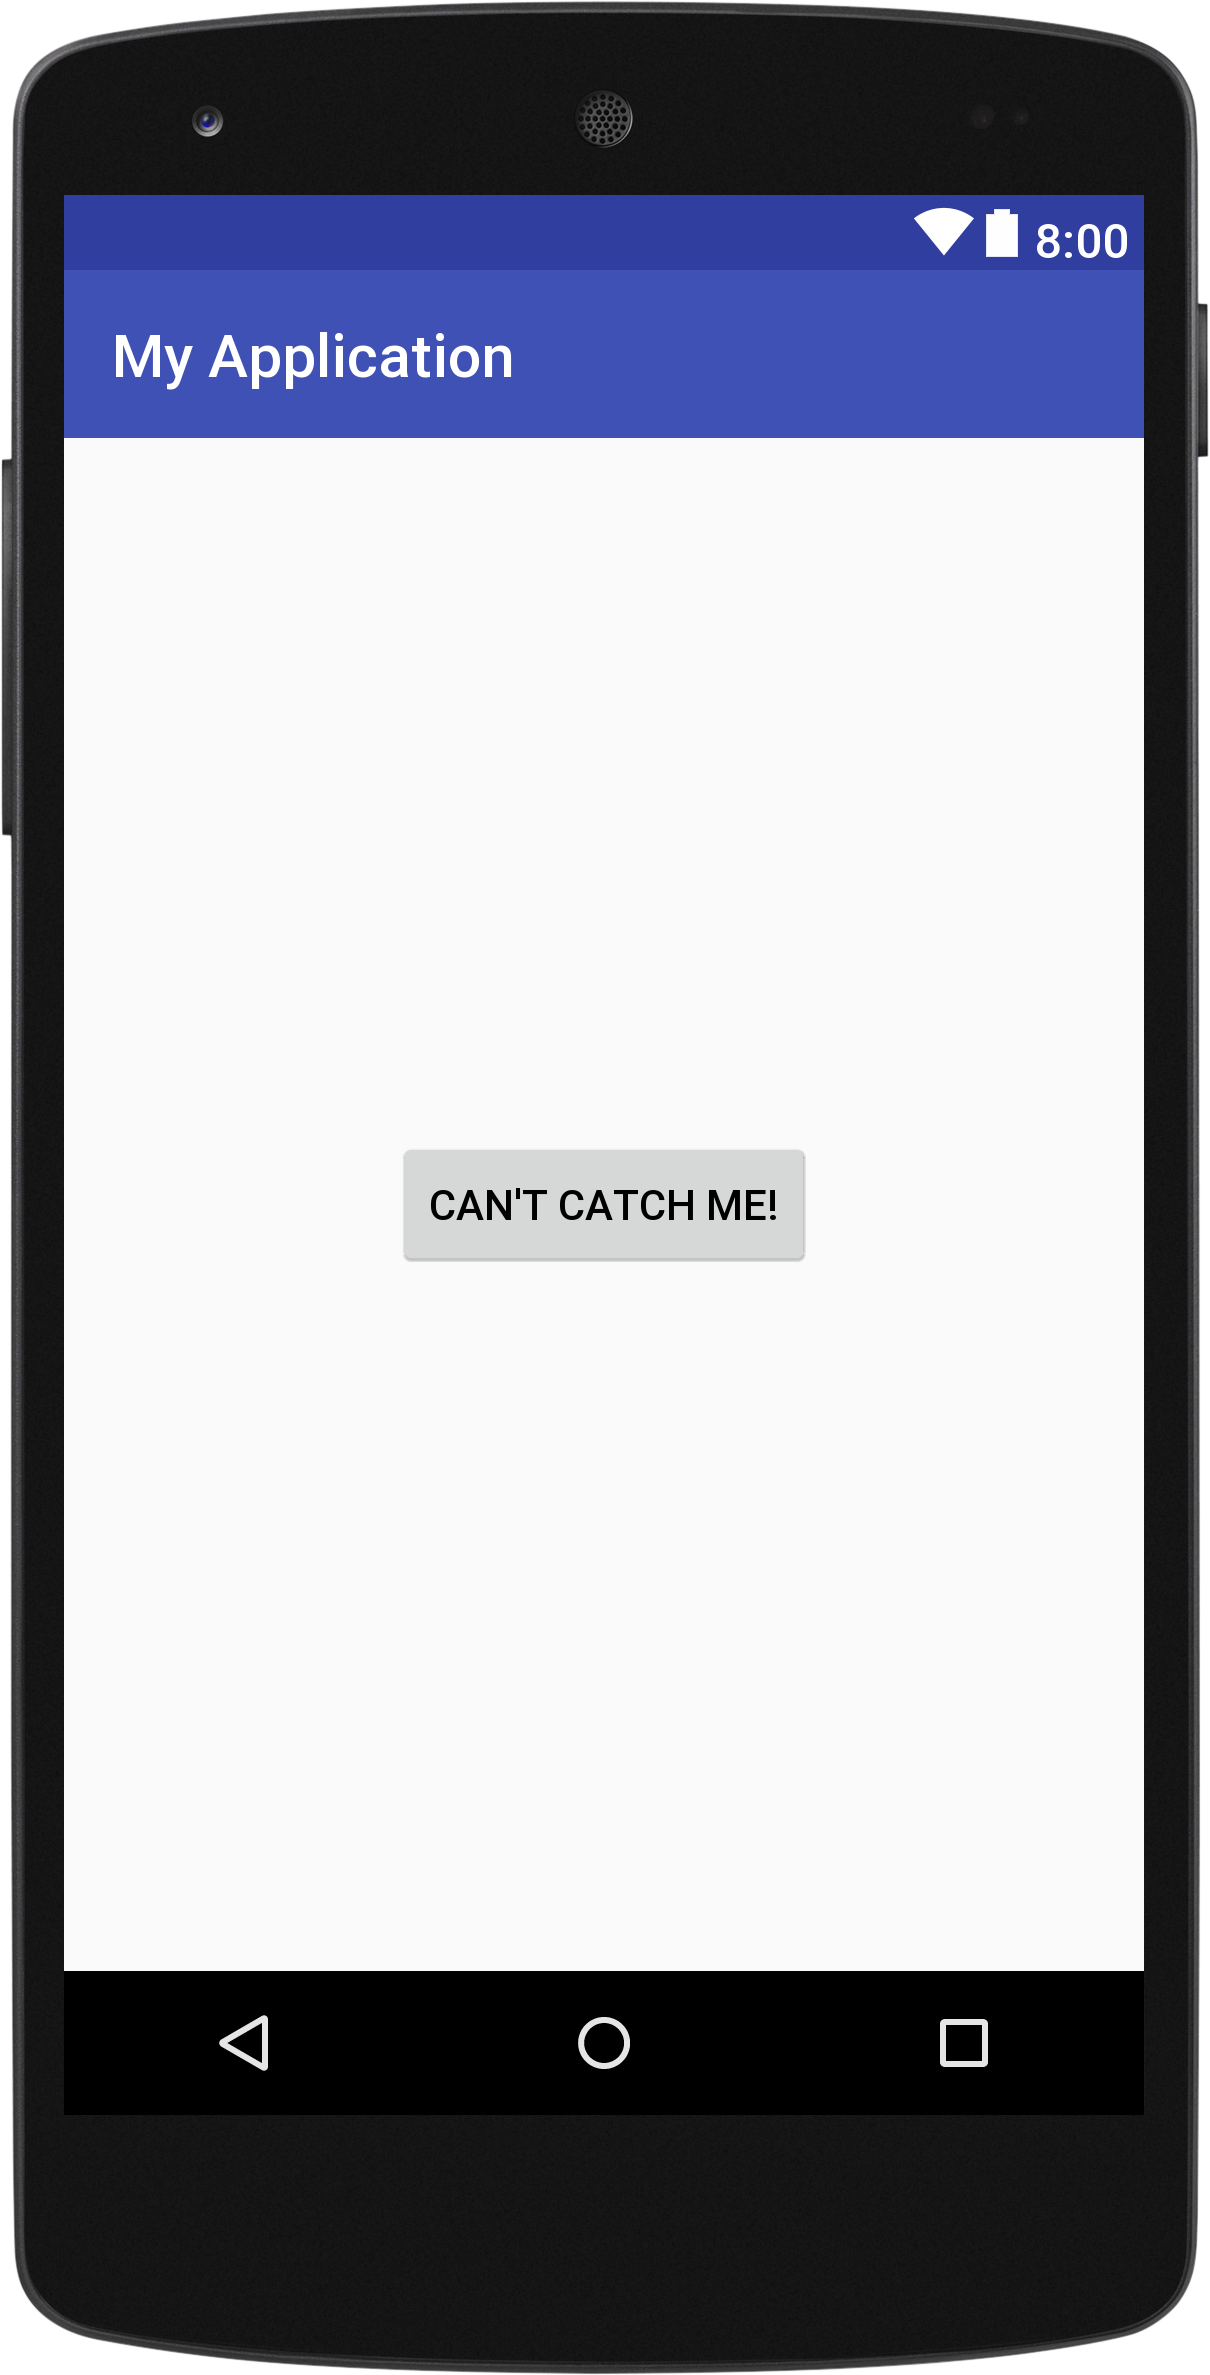
\includegraphics[width=5cm]{button_layout.png}
		\caption{Et relative layout med en knap i midten.}
		\label{fig:android:layouts:button-layout}
	\end{center}
\end{figure}

Hvis vi nu gerne vil have at app'en reagerer på, at vi trykker på denne knap, så 
kan vi tilføje ``android:onClick'' attributten til knappen, og give den attribut 
en værdi, der svarer til den funktion vi gerne vil have til at køre, når vi 
trykker på knappen. Et eksempel på dette kan ses i \autoref{lst:button-layout}.
Herefter kan vi blot tilføje den funktion vi tilføjede i ``onClick'' 
attributten til vores activity, som vist i \autoref{lst:button-activity}.

Vi kan se at ``buttonClicked'' funktionen får et ``View'' med som argument. 
Dette View er det element i app'ens \gls{interface}, der har udløst funktionen. 
I dette tilfælde er det knappen, man trykkede på. Hvis vi lægger $10$ til dens 
$x$ værdi, vil den flytte sig $10$ ``pixels'' til højre.

\begin{exercise}
	Implementér layoutet beskrevet i \autoref{lst:button-layout} og aktiviteten 
	i \autoref{lst:button-activity}.
\end{exercise}

\begin{exercise}
	Hvorfor skal vi lægge noget til $x$ for at flytte knappen mod højre? Hvad 
	betyder $x$?
\end{exercise}

\begin{exercise}
	Hvordan flytter man i stedet knappen op, ned eller til venstre?
\end{exercise}

\begin{exercise}
	Lav et layout med to knapper, den ene skal flytte sig op, når man trykker, 
	den anden skal flytte sig mod højre.
\end{exercise}

\clearpage


\begin{XmlCode}{Et layout med en knap, der kalder ``buttonClicked'' funktionen, % 
når den bliver trykket på.}{lst:button-layout}
	<?xml version="1.0" encoding="utf-8"?>
	<RelativeLayout 
		xmlns:android=
			"http://schemas.android.com/apk/res/android"
		xmlns:tools="http://schemas.android.com/tools"
		android:layout_width="match_parent"
		android:layout_height="match_parent"
		tools:context=
			"com.example.lukas.myapplication.MainActivity">
	
	<Button
		android:id="@+id/catchMeButton"
		android:layout_width="wrap_content"
		android:layout_height="wrap_content"
		android:layout_centerInParent="true"
		android:onClick="buttonClicked"
		android:text="Can't catch me!" />
		
	</RelativeLayout>
\end{XmlCode}

\clearpage

\begin{JavaCode}{En activity, der flytter en knap nedad, når den bliver trykket %
på.}{lst:button-activity}
	public class MainActivity extends AppCompatActivity {
		
		@Override
		protected void onCreate(Bundle savedInstanceState) {
			super.onCreate(savedInstanceState);
			setContentView(R.layout.activity_main);
		}
		
		
		public void buttonClicked(View view) {
			view.setX(view.getX() + 10);
		}
	}
\end{JavaCode}



	
	\graphicspath{{sections/android/activities/figures/}}
	% !TeX spellcheck = da_DK
\chapter{Activities og Intents}

Indtil videre har vi kigget kort på vores MainActivity som er entry point for en app. Hvis vi gerne vil have en ny activity, så skal vi starte denne med en intent. Dette kapitel vil kigge nærmere på en activity og dens livscyclus, forklare oprettelsen af nye activities, samt hvordan man kan starte disse activities med intents.

\section{Activities}

Dybere forklaring af MainActivity.

\subsection{Activity life cycle}

\begin{figure}[H]
	\begin{center}
		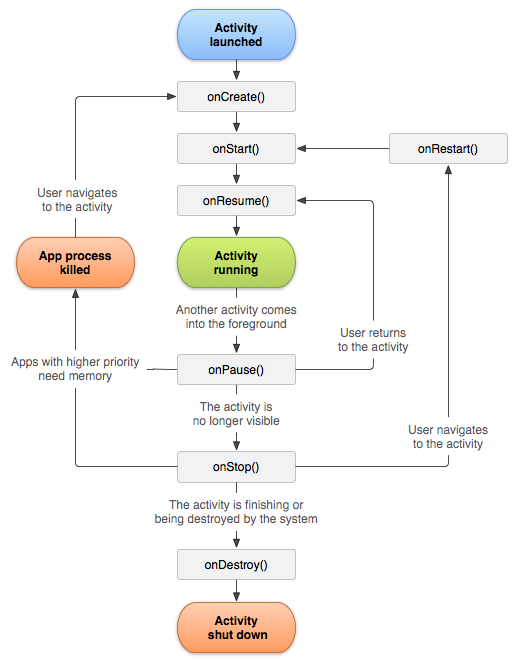
\includegraphics[width=7cm]{developerandroidcom_activitylifecycle.png}
		\caption{Activity lifecycle lånt af developer.android.com}
		\label{fig:android:activities:activitylifecycle}
	\end{center}
\end{figure}

Ovenstående figur viser de forskellige stadier en activity er i, og kan hjælpe til at give et overblik over hvornår de forskellige metoder bliver kaldt, og dermed også hvad man gerne vil have skal ske ide forskellige steps undervejs.

\subsection{Oprettelse af nye activities}

For at oprette en ny activity starter vi med at lave en ny java fil ved siden af MainActivity.java (i ??? folderen) En ny activity skal altid nedarve fra Activity, ligesom MainActivity. 

\begin{example}\noindent
	\begin{JavaCode}{Eksempel på en activity}{pop-up-activity}
		package com.example.housa.myapplication
		
		import android.app.Activity;
		import android.os.bundle;
		
		public class PopUpActivity extends Activity {
		  
		  @Override
		  protected void onCreate(Bundle savedInstanceState) {
		    super.onCreate(savedInstanceState);
		    setContentView(R.layout.activity_popup);
		  }
		}
	\end{JavaCode}
\end{example}

Ud over a skrive selve Java koden der definerer opførslen for en activity skal den til føjes til manifestet. Dette gøres ved at tilføje nedenstående kode til manifestet inde i application tag'et.

\begin{example}\noindent
	\begin{XmlCode}{XML der tilføjer PopUpActivity til manifestet}{add-activity-to-manifest}
		<activity android:name=".PopUpActivity" />
	\end{XmlCode}
\end{example}

For at kunne starte ovenstående activity skal vi benytte os af Intents som vil blive forklaret i næste sektion.


\section{Intents}

En intent er en besked man kan sende for at bede en anden komponent om at gøre noget. Intents kan bruges på flere forskellige måder, men de tre primære brugsscenarier er:

\subsubsection{Starte en anden activity}

Man kan starte en ny instans af en activity ved at sende en intent med som parameter til startActivity(). 

\subsubsection{Starte en service}

En service er et komponent der kører i baggrunden og ikke har noget interface. Man starter en service på lidt samme måde som en activity, nemlig ved at sende en intent med som parameter til metoden startService().

\subsubsection{Sende en broadcast}

En broadcast er en besked som enhver app kan modtage. Der er forskellelige broadcasts for system events som fx foretag opkald eller opladning igang. Man kan sende en broadcast ved at sende en intent med som parameter til sendBroadcast() eller sendOrderesBroadcast().
En standard broadcast kan ikke blive stoppet, og kan ikke videregive resultater. En orderedBroadcast vil sende broadcasten til alle relevante BroadCastRecievers en af gangen og tillade resultatet at propagere.

\subsection{Explicit vs Implicit}

Der er to typer intents explicitte og implicitte. I explicitte intents specificerer man præcist hvilket komponent man vil have til at reagere. Da man kender navngivningen i ens egen app, vil dette være den typeske måde at håndtere kommunikationen indenfor ens egen app, som at starte nye activities inde i appen.

De implicitte intents fortæller ikke præcist hvilket komponent man vil have til at reagere, men i stedet hvilken handling man gerne ville have udført, så kan alle komponenter der har den givne funktionalitet tilbyde at udføre handlingen. Dette benyttes fx hvis man gerne vil have ens app til at sende en mail, men gerne bare vil bruge hvad end mailklient brugeren allerede har på telefonen.

\subsection{Start en activity med en Intent}

hvordan det virker + hvor man gør det henne

eksempel kode

sende beskeder med intents

\subsection{Start en activity fra en anden app med en Intent}

implicit intents

eksempel kode på send mail der benytter indbygget mailklient

\subsection{Start en activity med en Intent fra en anden app}

modtag implicitte intents fra andre apps

broadcastrecievers


\begin{exercise}
	Lav en app der har en main activity, og en anden activity der viser et billede. Tilføj en knap til din main activity, der åbner din anden activity.
\end{exercise}

\begin{exercise}
	Lav en app der har en main activity, og en anden activity med et EditText felt. Tilføj en knap og et EditText felt til din main activity, der åbner din anden activity og viser teksten fra EditText i din main activity.
\end{exercise}

\begin{exercise}
	Lav en Activity der har en ‘send Emil’ knap, der åbner en Email dialog
\end{exercise}

\begin{exercise}
	Lav en activity der agerer som et alternativ til email klienten når man trykker på ‘send mail’ knappen fra opgave 3
\end{exercise}

\begin{exercise}
	Lav en BroadCastReciever, der blokerer alle udgående opkald.
\end{exercise}

\begin{exercise}
	Lav en activity der sender en Broadcast, og en BroadCastReciever der modtager den givne BroadCast.
\end{exercise}


	
	\graphicspath{{sections/android/animations/figures/}}
	% !TeX spellcheck = da_DK

\chapter{Animation}
Animation handler om at få ting til at bevæge sig og ændre udseende. Mere specifikt lærer I at få Views til at flytte sig på skærmen, rotere, ændre størrelse og på andre måder ændre udseende.
\section{Grundlæggende teori om animation}
Før vi går igang med at lave animationer i Android, skal vi lige have på plads, hvordan animationer virker.
Animationer og video er generelt en række af \gls{frame}s, som skifter så hurtigt, at det ligner en flydende bevægelse. \\
%TODO Illustration af still frames i række
Når man laver en animation foregår det altså ved, at man laver små ændringer i layoutet så hurtigt efter hinanden, at det bliver "flydende". En anden måde at sige det på er, at billedet ændrer sig i små hak, og man gør de hak så små, at det ikke kan ses, at der arbejdes i hak. Det vi skal lave er altså noget, der virker ligesom stopmotion. \\
Grunden til at man arbejder i hak er, at det tager en hel del arbejde for en computer \marginnote{En mobil er også en computer} at udregne, hvordan den skal vise et frame, så det gælder om at finde en balance mellem udseende, og hvor meget af computerens regnekraft animationen tager. Det animation vi arbejder med har nu et fastsat tempo for, hvor hurtigt billedet ændrer sig, så I skal ikke overveje denne balance.
\subsection{Animationens rammer}
En animation starter et sted og slutter på et andet sted. Det kan både være at ens view starter i bunden af skærmen og flytter sig til toppen, at den starter med at være lille og slutter med at være stor, eller at den starter på hovedet og roterer til den står lige.
Animationen tager også et stykke tid. Det kunne være et halvt sekund eller ti sekunder, det tager for den at nå fra start til slut. Her gælder det om at lave en balance mellem at animationen tager tid nok, så brugeren kan nå at se, hvad der sker, og at brugeren ikke sidder og venter på at animationen, bliver færdig. Hvis der ikke er stor forskel på start og slut i din animation kan det være at det slet ikke er nødvendigt at sætte en animation op, men bare at sætte dit View til slutpunktet med det samme. \marginnote{Hvis du bare vil have en oversigt over mulighederne for at ændre ens view så se sektionen "Hvad kan vi ændre"} \\
Ud fra disse rammer kan vi så regne, hvor langt vi skal være nået på et givet tidspunkt i animationen. 
\begin{example}
	Vi skal rykke et View fra 30 til 50 pixels horisontalt på 2 sekunder. Vi skal vide hvilken pixel vi er kommet til efter 0,5 sekunder, 1 sekund, 1,23 sekunder etc. Det vi kan gøre er, at plotte en funktion, hvilket er meget simpelt hvis den er lineær:
	\begin{equation}
	pixel=10\cdot tid+30
	\end{equation}
	Hvor 10 er antallet af pixels Viewet bevæger sig i sekundet og 30 er startværdien.
\end{example}
Vi skal nu ikke til at udregne en hel masse funktioner for animationen. Det gør Android for os.
\section{En helt simpel animation i Android}
For at lave en animation bruger vi den klasse, der hedder ValueAnimator. Du kan tænke på et objekt af ValueAnimator, som en animation. Du opretter en ValueAnimator som vist i \autoref{animation1}
\begin{JavaCode}{Oprettelse af ValueAnimator.}{animation1}
	ValueAnimator minAnimation = ValueAnimator.ofInt(startInt, slutInt);
\end{JavaCode}
\marginnote{Noter at du ikke skal skrive new. Den tekniske grund hertil er at ofInt() er en metode. som returnerer en ny ValueAnimator.}
ofInt() tager to integers, som er din startværdi og din slutværdi. Det kunne f.eks. være 0 og 360, hvis man ville animere et View til at rotere 360 grader. \\
Det næste din animation har brug for er, hvor lang tid den skal køre. Den sættes som vist i \autoref{animation2}
\begin{JavaCode}{Sæt duration}{animation2}
	minAnimation.setDuration(1000);	
\end{JavaCode}
Tiden er i millisekunder. Altså betyder 1000 et sekund. Fem sekunder ville være 5000 og et kvart sekund ville være 250. Værdien skal være et heltal.
\subsection{At lave en frame}
Nu har vi fortalt Android, hvor den skal starte og slutte, og hvor lang tid animationen skal tage. Nu skal vi så fortælle Android om den skal flytte noget, rotere noget eller gøre noget helt tredje. Dette gør vi ved at skrive en funktion, som bliver kaldt, hver gang billedet skal animeres endnu et hak. Altså skal vi programmere, hvad der sker hver gang, det er tid til en ny frame. Koden ser ud som i \autoref{animation3}
\begin{JavaCode}{Opsæt metode til at lave et frame.}{animation3}
	minAnimation.addUpdateListener(new ValueAnimator.AnimatorUpdateListener() {
		@Override
		public void onAnimationUpdate(ValueAnimator animation) {
			int vaerdiTilFrame = (int) animation.getAnimatedValue();
			
			mitView.setRotation(vaerdiTilFrame);
		}
	});
\end{JavaCode}
Her bruges noget advanceret kode, som I ikke behøver at forstå. Den korte version er at vi giver Android funktionen onAnimationUpdate() og fortæller ValueAnimator, at den skal kalde funktionen, når den vil have en ny frame.\\
\marginnote{Hvis I vil have den længere udgave, så spørg os eller internettet om anonyme klasser}
Den anden ting, der sker er, at vi får en integer fra animationen, som repræsenterer hvor langt vi er i animationen. Det er den variabel, der hedder "vaerdiTilFrame" som man får fra getAnimatedValue(). Vi udfører så ændringen på vores view med denne værdi, i eksemplet sætter vi rotationen med setRotation, men I kan bruge denne værdi til lige, hvad I vil. De mulige måder at ændre views på kommer om lidt.\\
Til sidst skal du kalde .start() på din ValueAnimator, og så kører animationen. Et fuldt eksempel på en animation kan ses i \autoref{animation4}
\begin{JavaCode}{420 Rotate it}{animation4}
	ValueAnimator minAnimation = ValueAnimator.ofInt(0, 420);
	minAnimation.setDuration(1337);
	minAnimation.addUpdateListener(new ValueAnimator.AnimatorUpdateListener() {
		@Override
		public void onAnimationUpdate(ValueAnimator animation) {
			int vaerdiTilFrame = (int) animation.getAnimatedValue();
			mitView.setRotation(vaerdiTilFrame);
		}
	});
	minAnimation.start();
\end{JavaCode}
I kan nu lave animationer i Android. Huzzah!

\section{Flere grundteknikker}
Nu hvor det helt basale er på plads, kan vi udvide med nogle flere teknikker
\subsection{Brug af decimaltal}
Man kan også oprette en ValueAnimator som bruger decimaltal i form af typen float istedet for at bruge int. Koden til dette ses i \autoref{animationfloat}
\begin{JavaCode}{decimaltal}{animationfloat}
	ValueAnimator minAnimation = ValueAnimator.ofFloat(0.0, 1.0);
\end{JavaCode}
På denne måde kan man få noget mere præcist animation istedet for at alting afrundes til heltal.

\subsection{Hvad kan vi ændre}
Her er der så en liste over, hvad man kan lave med Views:\\
\begin{itemize}
	\item View rotation
	I kan sætte et views rotation som i \autoref{animationroter}.
	\begin{JavaCode}{Roter et view.}{animationroter}
		mitView.setRotation(jeresRotation);
	\end{JavaCode}
	Rotationen er i grader. 0 er normal rotation og 180 grader er på hovedet. Rotationen er en float. 
	\\
	\item View position
	Her sættes vertikal og horizontal position seperat. Koden ses i \autoref{animationflyt}
	\begin{JavaCode}{Flyt et view.}{animationflyt}
		mitView.setX(jeresPositionX);
		mitView.setY(jeresPositionY);
	\end{JavaCode}
	Her skal det noteres at det er \textbf{øverste} venstre hjørne, der er position (0,0). Ligeledes er det viewets øverste venstre hjørne der placeres. Hvis I vil placere et view op af skærmens højre side, skal i altså sætte X til skærmbredden minus viewets bredde. I kan få bredden og højden af jeres view som i \autoref{animationbredde}.
	\begin{JavaCode}{Få bredden af jeres view.}{animationbredde}
		mitView.getWidth();
		mitView.getHeight();
	\end{JavaCode}
	Man kan også placere et views position ud fra at (0,0) er viewets startposition med funktionerne getTranslationX() og getTranslationY().
	\item View størrelse
	I kan sætte størrelsen som i \autoref{animationscale}.
	\begin{JavaCode}{Sæt størrelsen af jeres view.}{animationscale}
		mitView.setScaleX(jeresStoerlseX);
		mitView.setScaleY(jeresStoerlseY);
	\end{JavaCode}
	Her er 1 den størrelse, som viewet starter med. Skal størrelsen fordobles, skal I give slutværdien 2. Skal den halveres, skal I give slutværdi 0.5 etc. Hvis i vil sætte størrelsen til et præcist antal pixels, skal i lave en udregning ud fra viewets nuværende størrelse. \\
	\item View gennemsigtighed
	Et view kan gøres gennemsigtigt (Man kan stadig interagere med det) med metoden set i \autoref{animationgennemsigtig}.
	\begin{JavaCode}{Sæt et views gennemsigtighed.}{animationgennemsigtig}
		mitView.setAlpha(jeresGennemsigtighed);
	\end{JavaCode}
	Her er 0 usynlig og 1 er fuldt synlig. Værdien som tages, er selvfølgelig en float.
\end{itemize}
\subsection{Størrelsen af skærmen}
Der findes mange forskellige Android mobiler, og de har mange forskellige skærmstørrelser, især hvis man også arbejder med tablets. 
\begin{example}
	Den mobil I arbejder med, har en skærmbredde på 480 pixels. I har et view, som skal krydse skærmen og det sættes til at starte i 0 og bevæge sig 480 pixels. Og det virker lige som det skal på jeres test mobil. I prøver så at køre appen på en tablet med en skærmbredde på 1080 pixels. Jeres view når ikke engang halvvejs over skærmen. 
\end{example}
Det gælder derfor om altid at arbejde ud fra skærmens størrelse. Jeres view i eksemplet skal bevæge sig en hel skærmbredde. En figur, som står i baggrunden og hopper skal hoppe 1/3 af skærmhøjden. Etc.\\

Og siden skærmstørrelsen er så kritisk skulle man tro at den var lettere at få fat på. Men nej, koden for at få skærmstørrelsen ser ud som i \autoref{animation5}
\begin{JavaCode}{Kode til at få skærmstørrelse.}{animation5}
	//Inde i onCreate()
	final View layout = findViewById(R.id.layout);
	ViewTreeObserver observer = layout.getViewTreeObserver();
	observer.addOnGlobalLayoutListener(new ViewTreeObserver.OnGlobalLayoutListener() {
		@Override
		public void onGlobalLayout() {
			screenHeight = layout.getHeight();
			screenWidth = layout.getWidth();
			//kode der bruger height og width her
			layout.getViewTreeObserver().removeOnGlobalLayoutListener(this);
		}
	});
\end{JavaCode}

I skal også give jeres yderste layout et ID og hente det med findViewByID(). Så skal i have screenHeight og screenWidth, som feltvariabler. Hvis I skal bruge størrelsen af skærmen i onCreate(), skal den kode også stå inde i onGlobalLayout().
Grunden hertil er, at Android ikke har udregnet hvordan grafikken placeres, når OnCreate bliver kaldt. Vi får den så til at kalde onGlobalLayout når den har fundet størrelsen af layoutet.
\subsection{Interpolatorer}
Det, vi har defineret for Android, er egentlig kun startpunkt, slutpunkt og tid imellem dem. Hvordan funktionen mellem de to punkter ser ud kan også defineres. Det kan være at den bare er lineær, men den kunne også være en exponentiel funktion, hvor hastigheden starter med at være langsom og så derefter bliver hurtigere. Man styrer dette ved at sætte en interpolator. 
Hvis du ikke sætter en interpolator, så vil Android bruge AccelerateDecelerateInterpolator. Altså vil hastigheden for animationen være langsommere i starten og slutningen og så være hurtig i midten. Du sætter en interpolator som i \autoref{animation6}
\begin{JavaCode}{Kode til at sætte interpolatoren}{animation6}
	animator.setInterpolator(new LinearInterpolator());
\end{JavaCode}

Du kan sætte interpolatoren mellem, at du opretter animationen og starter den.
De helt basale muligheder er LinearInterpolator, AccelerateInterpolator, DecelerateInterpolator og så selvfølgelig AccelerateDecelerateInterpolator. Der findes dog flere, som man kan finde online.
%TODO Illustrationer til interpolators
\subsection{Kontrolmetoder}
Animator har yderligere en række metoder, som gør den lettere at arbejde med. Du kan sætte animationen til først at starte noget tid efter at du kalder .start() ved at kalde koden i \autoref{animation7}. \\
\begin{JavaCode}{Kode til at sætte et startDelay}{animation7}
	minAnimation.setStartDelay(minForsinkelse);
\end{JavaCode}
Forsinkelsen er igen i millisekunder, præcist som setDuration. 
Yderligere er der metoderne .pause(), .resume(), .cancel(),  .end() og .reverse(), som meget vel giver sig selv. .end() sætter animationen til slutværdien, og .cancel() efterlader den hvor den er nået til.
\section{Mere advancerede teknikker}
Her kommer vi omkring nogle lidt mere advancerede teknikker.
\subsection{Flere animationer samlet}
Vi kan samle flere animationer i en, så vi kan flytte vores view diagonalt, eller få det til at ændre farve og rotere samtidigt. Til dette bruger vi AnimatorSet. Det virker som set i \autoref{animation8}:
\begin{JavaCode}{Kode til at køre flere animationer samtidigt.}{animation8}
AnimatorSet mitAnimationSet = new AnimatorSet();
mitAnimatorSet.playTogether(minAnimation, minAndenAnimation);
mitAnimatorSet.start();
\end{JavaCode}
Vi laver altså et AnimatorSet, og så kalder vi .playTogether() med vores animationer som argumenter. Derefter starter vi vores sæt af animationer. Her skal det noteres at AnimatorSet opfører sig meget ligesom ValueAnimator, og man kan stadig pause den og give den et startDelay m.m. 
Desuden kan man lave et AnimatorSet af andre AnimatorSets. Altså give et AnimatorSet som parameter til .playTogether(). Man kan desuden give playTogether lige så mange animationer, som man har lyst til.
%Muligvis kortere navne til argumenter så linjen kan være i bogen
\begin{JavaCode}{Køre mange animationer samlet.}{animation9}
	mitAnimatorSet.playTogether(minAnimation, minAndenAnimation, rotation, hop);
\end{JavaCode}

\subsection{Animationer i rækkefølge}
Vi kan også spille animationer efter hinanden. Her bruger vi igen AnimatorSet, som ses i \autoref{animation10}
\begin{JavaCode}{Kode til at køre flere animationer efter hinanden.}{animation10}
	AnimatorSet mitAnimationSet = new AnimatorSet();
	mitAnimatorSet.playSequentially(minAnimation, minAndenAnimation);
	mitAnimatorSet.start();
\end{JavaCode}
Så kører minAnimation først og derefter kører minAndenAnimation. Igen kan man give lige så mange animationer, som man vil. 
%igen, muligvis forkort argument navne for at passe koden til siden
\begin{JavaCode}{Kør mange animationer efter hinanden.}{animationer11}
	mitAnimatorSet.playSequentially(minAnimation, minAndenAnimation, minTrejdeAnimation);
\end{JavaCode}
\subsection{Gentagelser}
Vi kan også sætte vores animationer til at gentage. Det er meget simpelt, se \autoref{animation12}.
\begin{JavaCode}{Kode til at lave gentagelser.}{animation12}
	minAnimation.setRepeatCount(antalGentagelser);
\end{JavaCode}
Her er det værd at notere, at hvis man sætter antalGentagelser til 2, så afspiller animationen \textbf{3 gange} i alt. Den gentager 2 gange.
Man kan også sætte gentagelsen som i \autoref{animation13}.
\begin{JavaCode}{Sæt animationen til at køre tilbage.}{animation13}
	minAnimation.setRepeatMode(ValueAnimator.REVERSE);
\end{JavaCode}
Hvilket gør at den på gentagelsen ikke går tilbage og kører forfra, men går fra slutværdien til startværdien. Den vil så igen gå fra start til slut på anden gentagelse etc.

\section{Hurtig guide}
Her er en lille 4 skridts guide til at lave en animation.
\begin{enumerate}
	\item Opret en ValueAnimator med enten ofInt() eller ofFloat() \autoref{animationguide1}.
	\begin{JavaCode}{Opret animator}{animationguide1}
	ValueAnimator minAnimation = ValueAnimator.ofFloat(startFloat, slutFloat);
	\end{JavaCode}
	\item Sæt en varighed i millisekunder \autoref{animationguide2}.
	\begin{JavaCode}{Sæt varighed}{animationguide2}
	minAnimation.setDuration(varighed);
	\end{JavaCode}
	\item Lav onAnimationUpdate og få den til at lave din ændring \autoref{animationsguide3}.
	\begin{JavaCode}{Lav et billede}{animationsguide3}
		minAnimation.addUpdateListener(new ValueAnimator.AnimatorUpdateListener() {
			@Override
			public void onAnimationUpdate(ValueAnimator animation) {
				int vaerdiTilBillede = (int) animation.getAnimatedValue();
				//Manipuler dit view her
				mitView.setScale(vaerdiTilBillede);
			}
		});
	\end{JavaCode}
	\item Start animationen \autoref{animationguide4}.
	\begin{JavaCode}{Start animationen}{animationguide4}
		minAnimation.start();
	\end{JavaCode}
\end{enumerate}

\subsubsection{Animationsopgaver}
Der er ingen tid afsat til specifikt at lave opgaver i animation, men programmering er et praktisk fag, så det gælder om at øve sig. Her er nogle forslag til ting at øve sig med, men du kan også selv finde på udfordringer at øve dig på, inklusiv bare at gå direkte i gang med projektet. Hvis det ikke går godt så husk, at tage små skridt og lave én ting af gangen.
\begin{exercise}
	Start helt fra bunden. Få en knap til at rotere 360 grader, når du trykker på den.
\end{exercise}
\begin{exercise}
	Giv rotationen et startdelay, så der går et øjeblik, før den begynder at rotere.
\end{exercise}
\begin{exercise}
	Sæt din knap til at starte i venstre side af skærmen og så bevæge sig til midt på skærmen, når du trykker på den.
\end{exercise}
\begin{exercise}
	Sæt bevægelsens interpolator til at være lineær.
\end{exercise}
\begin{exercise}
	Kombinér de to første animationer, så knappen først bevæger sig sidelæns og så derefter roterer
\end{exercise}
\begin{exercise}
	Sæt nu knappen til at starte i øverste højre hjørne. Få den til at bevæge sig lodret og vandret samtidigt til midt på skærmen, og derefter rotere en omgang. Noter hvordan, den lodrette bevægelse starter og slutter langsomt fordi den bruger den normale interpolator, mens den horizontale bevægelse er lineær
\end{exercise}
\begin{exercise}
	Få rotationen til at gentage sig selv 2 gange. Sæt derefter dens repeatMode til at være reverse.
\end{exercise}
\begin{exercise}
	Lav en knap, som bevæger sig yderligere 10 pixels til højre, hver gang man trykker på den. Hint: Her ændrer startInt sig for hver animation.
\end{exercise}
\begin{exercise}
	Få helt styr på at arbejde med skærmens størrelse. Placer en knap i øverste venstre hjørne og få den til at tage en fuld runde langs telefonens kant, når du trykker på den. 
\end{exercise}

%Ordliste
%Frame
	
	\ifdraftmode
		\glsaddall
	\fi
	\printglossary
	
	%% Indsæt ``indexet'' som er et overblik over emner bogen indeholder, der 
	%% skabes ved hjælp af \index makroen.
	\cleardoublepage
\phantomsection
\setlength{\columnsep}{0.75cm}
\addcontentsline{toc}{chapter}{\textcolor{ocre}{Index}}
\printindex

\end{document}
